% ══════════════════════════════════════════════════════════════════
% RAPPORT PFE — AGRO-IA TCHAD — ENASTIC 2025/2026
% TOURABI ISSAK HISSEIN
% Agencement (plan de travail adopté) :
% Page de garde · Dédicaces · Remerciements · Résumé · Abstract ·
% Sommaire · Liste figures · Liste tableaux · Abréviations ·
% Introduction générale · Chapitres 1-4 · Conclusion générale ·
% Bibliographie · Annexes A-D · Table des matières
% ══════════════════════════════════════════════════════════════════

\documentclass[12pt,a4paper,oneside]{report}
% ══════════════════════════════════════════════════════════════════
% PREAMBULE — Tous les packages du rapport (règles du guide ENASTIC)
% Police Times New Roman 12pt · Marges 2cm · Interligne 1,5 · Justifié
% ══════════════════════════════════════════════════════════════════

% ── Encodage & langue ─────────────────────────────────────────────
\usepackage[utf8]{inputenc}
\usepackage[T1]{fontenc}
\usepackage[french]{babel}
\usepackage{csquotes}

% ── Police Times New Roman (règle 2 du guide) ────────────────────
\usepackage{mathptmx}          % Times New Roman texte + maths

% ── Marges : 2cm partout (règle 2 du guide) ──────────────────────
\usepackage[top=2cm,bottom=2cm,left=2cm,right=2cm]{geometry}
\setlength{\headheight}{15pt}

% ── Interligne 1,5 (règle 2 du guide) ────────────────────────────
\usepackage{setspace}
\onehalfspacing

% ── Paragraphes justifiés (défaut LaTeX) + retrait ───────────────
\usepackage{microtype}
\setlength{\parindent}{1cm}

% ── Couleurs ──────────────────────────────────────────────────────
\usepackage{xcolor}
\usepackage[most]{tcolorbox}
\usepackage[dvipsnames,table]{xcolor}
\definecolor{bleuENASTIC}{RGB}{55,90,170}   % bleu bordure page garde
\definecolor{grisbleu}{RGB}{70,90,110}
% Couleurs pastel des diagrammes UML
\definecolor{vertdiag}{RGB}{225,240,225}
\definecolor{bleudiag}{RGB}{222,235,250}
\definecolor{jaunediag}{RGB}{253,246,220}
\definecolor{rougediag}{RGB}{250,228,225}
\definecolor{violetdiag}{RGB}{238,230,248}

% ── Graphiques ────────────────────────────────────────────────────
\usepackage{graphicx}
\usepackage{float}
\usepackage{tikz}
\usetikzlibrary{arrows.meta,shapes.geometric,positioning,fit,backgrounds,calc}

% ── Tableaux ──────────────────────────────────────────────────────
\usepackage{booktabs}
\usepackage{tabularx}
\usepackage{multirow}
\usepackage{longtable}
\usepackage{array}

% ── Encadrés ──────────────────────────────────────────────────────
\usepackage{mdframed}

% ── Listes ────────────────────────────────────────────────────────
\usepackage{enumitem}

% ── Mathématiques ─────────────────────────────────────────────────
\usepackage{amsmath,amssymb}

% ── Code source ───────────────────────────────────────────────────
\usepackage{listings}
\definecolor{codebg}{rgb}{0.97,0.97,0.97}
\definecolor{codeblue}{rgb}{0,0,0.8}
\definecolor{codegreen}{rgb}{0,0.5,0}
\definecolor{codepurple}{rgb}{0.5,0,0.5}
\definecolor{codegray}{rgb}{0.5,0.5,0.5}
\lstset{
	backgroundcolor=\color{codebg},
	basicstyle=\ttfamily\small,
	keywordstyle=\color{codeblue}\bfseries,
	commentstyle=\color{codegreen}\itshape,
	stringstyle=\color{codepurple},
	numberstyle=\tiny\color{codegray},
	numbers=left,numbersep=8pt,
	frame=single,breaklines=true,
	tabsize=4,showstringspaces=false,
	captionpos=b,language=Python
}

% ── Abréviations ──────────────────────────────────────────────────
\usepackage{acronym}

% ── Hyperliens ────────────────────────────────────────────────────
% Liens cliquables : citations [n] en bleu -> bibliographie,
% URL/DOI en bleu -> consultation directe en ligne,
% ET numeros de page du Sommaire/listes cliquables (linktoc=all)
\definecolor{bleuLien}{RGB}{0,60,160}
\usepackage[colorlinks=true,
linkcolor=black,        % renvois internes (sections, figures)
citecolor=bleuLien,     % citations [1] cliquables et visibles
urlcolor=bleuLien,      % URL et DOI cliquables
linktoc=all,            % Sommaire/listes : titre ET numero de page cliquables
bookmarksnumbered=true, % signets PDF numerotes (1, 1.1, 1.2...)
bookmarksopen=true]{hyperref}

% ── En-têtes / pieds de page ──────────────────────────────────────
\usepackage{fancyhdr}
\usepackage{emptypage}
\pagestyle{fancy}
\fancyhf{}
\fancyhead[L]{\small\leftmark}
\fancyhead[R]{\small PFE Licence --- 2025/2026}
\fancyfoot[C]{\thepage}
\renewcommand{\headrulewidth}{0.4pt}

% ── Bibliographie IEEE ────────────────────────────────────────────
% hyperref=true : citations [n] du corps cliquables -> bibliographie ;
% backref=false ; les champs url/doi de chaque entrée sont cliquables -> site
\usepackage[backend=biber,style=ieee,sorting=none,
hyperref=true,defernumbers=false]{biblatex}
\addbibresource{references.bib}

% ── Légendes : figure DESSOUS, tableau DESSUS (règle 3) ──────────
\usepackage{caption}
\captionsetup[figure]{labelfont=bf,labelsep=colon,position=below}
\captionsetup[table]{labelfont=bf,labelsep=colon,position=above}

% ── Numérotation Figure 2.4 / Tableau 1.5 (règle 3) ──────────────
\numberwithin{figure}{chapter}
\numberwithin{table}{chapter}
\numberwithin{equation}{chapter}

% ── CHAPITRES EN MAJUSCULES, SEULS AU CENTRE D'UNE PAGE (règle 1) ─
\usepackage{titlesec}
% Le titre du chapitre : taille 14, MAJUSCULES, centré sur page vierge
\titleformat{\chapter}[display]
{\normalfont\centering}
{\fontsize{14}{18}\selectfont\bfseries\MakeUppercase{\chaptertitlename}~\thechapter}
{12pt}
{\fontsize{14}{18}\selectfont\bfseries\MakeUppercase}
\titlespacing*{\chapter}{0pt}{0.32\textheight}{20pt}

% Commande : titre du chapitre SEUL au centre d'une page vierge
% (règle 1 du guide) — le contenu commence à la page suivante.
% Usage : \pagechapitre{chap:label}{Titre du chapitre}
\newcommand{\pagechapitre}[2]{%
	\clearpage
	\chapter{#2}\label{#1}%
	\thispagestyle{empty}%
	\vspace*{\fill}%
	\clearpage
}

\begin{document}
	
	% ═══════════════ ÉLÉMENTS LIMINAIRES (numérotation romaine) ══════
	\pagenumbering{roman}
	
	% 1) Page de garde
	% ══════════════════════════════════════════════════════════════════
% PAGE DE GARDE — modèle ENASTIC (fragment, inclus par main.tex)
% ══════════════════════════════════════════════════════════════════

\begin{titlepage}
	\thispagestyle{empty}
	
	% ── Bordure bleue extérieure (comme le modèle) ───────────────────
	\begin{tikzpicture}[remember picture, overlay]
		\draw[bleuENASTIC, line width=1.6pt]
		([xshift=0.9cm,  yshift=-0.9cm] current page.north west) rectangle
		([xshift=-0.9cm, yshift=0.9cm]  current page.south east);
	\end{tikzpicture}
	
	% ── Logos : ENASTIC à gauche, institution d'accueil à droite ─────
	
	\vspace{-1cm}
	\noindent
	\begin{minipage}[t]{2\textwidth}
		\vspace{0pt}
		% Placez votre logo dans images/logo_enastic.png
		\IfFileExists{images/logo_enastic.png}{%
			
\includegraphics[width=11cm]{images/logo_enastic.png}%
		}{%
			{\Large\bfseries\color{bleuENASTIC}ENASTIC}\\[2pt]
			{\footnotesize École Nationale Supérieure des TIC}%
		}
	\end{minipage}

	
	% ── Titre principal ───────────────────────────────────────────────
	\begin{center}
		{\fontsize{28}{34}\selectfont\bfseries Projet de Fin d'Études}
		
		\vspace{1cm}
		
		{\large En vue de l'obtention du Diplôme de Licence en Informatique}
		
		\vspace{0.5cm}
		
		{\large \textbf{Option} : Informatique}
		
	\vspace{0.1cm}
		
		% ── Encadré THÈME ─────────────────────────────────────────────────
\begin{tcolorbox}[
	enhanced,
	colback=white,
	colframe=blue,
	boxrule=2pt,
	arc=5mm,
	width=\textwidth,
	center title,
	left=6mm,
	right=6mm,
	top=5mm,
	bottom=5mm
	]
	
	\begin{center}
		
		{\LARGE\bfseries THÈME : }
		
		\vspace{0.4cm}
		
		{\Large\bfseries
			Conception et Implémentation d'un Cadre Décisionnel\\[0.35cm]
			basé sur l'Intelligence Artificielle pour l'Optimisation\\[0.35cm]
			du Suivi Parcellaire Agricole au Tchad\\[0.5cm]
			\large (Irrigation, Fertilisation et Détection des Maladies)
		}
		
	\end{center}
	
\end{tcolorbox}
	\vspace{1.6cm}
	
	% ── Rédigé par / Sous la Direction de ─────────────────────────────
	\noindent
	\begin{minipage}[t]{0.46\textwidth}
		\underline{\textbf{Rédigé et Présenté par}} :\\[10pt]
		TOURABI ISSAK HISSEIN
	\end{minipage}
	\hfill
	\begin{minipage}[t]{0.50\textwidth}
		\underline{\textbf{Sous la Direction de}} :\\[10pt]
		Dr. MOUAZ MIKAIL ,\\
		Enseignant Chercheur à ENASTIC
	\end{minipage}
	
	\vspace{1.8cm}
	
	% ── Jury ──────────────────────────────────────────────────────────
	\noindent\underline{\textbf{Jury}} :\\
	\ldots\ldots\ldots\ldots\ldots\ldots\ldots\ldots\ldots\ldots\ldots \ldots\ldots\ldots\ldots\ldots\ldots\ldots\ldots\ldots\ldots\ldots
	\ (Président)\\[6pt]
	\ldots\ldots\ldots\ldots\ldots\ldots\ldots\ldots\ldots\ldots\ldots \ldots\ldots\ldots\ldots\ldots\ldots\ldots\ldots\ldots\ldots\ldots
	\ (Rapporteur)
	
	\vfill
	
	% ── Année académique dans une ellipse ─────────────────────────────
	\begin{center}
		\begin{tikzpicture}
			\node[draw=black, line width=0.9pt, ellipse,
			inner xsep=18pt, inner ysep=6pt]
			{\textbf{Année Académique 2025--2026}};
		\end{tikzpicture}
	\end{center}
	
\end{titlepage}
	
	% 2) Dédicaces
	% ══════════════════════════════════════════════════════════════════
% DÉDICACE
% ══════════════════════════════════════════════════════════════════

\chapter*{Dédicace}
\addcontentsline{toc}{chapter}{Dédicace}
\thispagestyle{empty}

\vspace*{3cm}

\begin{flushright}
\begin{minipage}{0.6\textwidth}
\itshape

\textit{À mes chers parents,}\\[0.5cm]
\textit{pour leur amour inconditionnel,}\\
\textit{leurs sacrifices et leur soutien indéfectible}\\
\textit{tout au long de mon parcours académique.}\\[1cm]

\end{minipage}
\end{flushright}

	\newpage
	
	% 3) Remerciements
	% ══════════════════════════════════════════════════════════════════
% REMERCIEMENTS
% ══════════════════════════════════════════════════════════════════

\chapter*{Remerciements}
\addcontentsline{toc}{chapter}{Remerciements}
\thispagestyle{plain}

Au terme de ce travail, il m'est agréable d'exprimer ma profonde
gratitude envers toutes les personnes qui ont contribué, de près
ou de loin, à sa réalisation.

\medskip

Mes premiers remerciements vont à \textbf{Dr. MOUAZ MIKAIL},
mon encadreur, pour sa disponibilité permanente, ses précieux
conseils scientifiques et sa rigueur méthodologique qui ont
grandement orienté la conduite de ce travail. Sa patience et
son expertise ont été une source d'inspiration tout au long de
cette expérience.

\medskip

Je remercie sincèrement les membres du jury qui ont accepté
d'évaluer ce travail et d'apporter leurs critiques constructives
pour son amélioration.

\medskip

Ma gratitude va également à l'ensemble du corps enseignant et
administratif de l'\textbf{École Nationale Supérieur des TIC (ENASTIC)} pour la qualité de
la formation académique et professionnelle qu'ils m'ont dispensée
durant mon cursus.

\medskip

Je tiens à remercier chaleureusement mes camarades de promotion
pour l'ambiance studieuse et fraternelle, ainsi que les échanges
enrichissants qui ont jalonné notre formation.

\medskip

Enfin, mes remerciements les plus profonds vont à ma famille,
en particulier à mes parents et à mon oncle HASSAN HISSEIN DAOUD, pour leur soutien moral et matériel
indéfectible, et pour tous les sacrifices consentis afin de
permettre la réussite de mes études.

\medskip

Que tous ceux dont le nom ne figure pas ici, mais qui ont
contribué d'une manière ou d'une autre à l'élaboration de
ce mémoire, trouvent ici l'expression de ma sincère
reconnaissance.

	\newpage
	
	% 4) Résumé + Abstract
	% ══════════════════════════════════════════════════════════════════
% RÉSUMÉ (français) + ABSTRACT (anglais)
% ══════════════════════════════════════════════════════════════════

\chapter*{Résumé}
\addcontentsline{toc}{chapter}{Résumé}
\markboth{Résumé}{Résumé}
\thispagestyle{plain}

L'agriculture tchadienne, pilier de l'économie nationale, souffre
d'un déficit d'outils d'aide à la décision adaptés aux réalités
locales. Ce mémoire présente la conception et l'implémentation
d'un cadre décisionnel basé sur l'Intelligence Artificielle pour
l'optimisation du suivi parcellaire agricole au Tchad, dénommé
\textbf{Agro-IA Tchad}.

\medskip

Le système intègre quatre modules complémentaires. Le
\textbf{module Irrigation} repose sur l'algorithme Random Forest,
entraîné sur 16~435 observations climatiques réelles issues de la
base NASA POWER pour cinq villes tchadiennes (2015--2023) ; il
atteint une accuracy de 78,51\,\% et un AUC-ROC de 0,8782. Le
\textbf{module Fertilisation} utilise XGBoost sur 1~599
observations et recommande l'engrais optimal avec une accuracy de
95,42\,\% (F1-score macro de 95,47\,\%). Le \textbf{module
	Détection des maladies} combine un réseau de neurones convolutif
MobileNetV2 --- entraîné par transfert d'apprentissage sur un
dataset local de 287 images de cultures tchadiennes (accuracy de
52,27\,\%) --- avec l'analyse d'indices de végétation NDVI issus
du satellite Sentinel-2 ou estimés par caméra smartphone (indice
VARI). Enfin, le \textbf{module Historique} assure la traçabilité
de toutes les analyses grâce à une base de données SQLite avec
export CSV.

\medskip

L'application web, développée avec le framework Streamlit et
intégrant l'API météorologique Open-Meteo en temps réel, est
déployée sur Streamlit Cloud et accessible depuis tout navigateur.

\medskip

\noindent\textbf{Mots-clés :} Intelligence Artificielle, Random
Forest, XGBoost, CNN MobileNetV2, NDVI, Agriculture de précision,
Tchad, Streamlit, SQLite.

\newpage

% ──────────────────────────────────────────────────────────────────
\chapter*{Abstract}
\addcontentsline{toc}{chapter}{Abstract}
\markboth{Abstract}{Abstract}
\thispagestyle{plain}

Chadian agriculture, a pillar of the national economy, suffers
from a lack of decision-support tools adapted to local realities.
This thesis presents the design and implementation of an
Artificial Intelligence-based decision framework for optimizing
agricultural plot monitoring in Chad, named \textbf{Agro-IA
	Tchad}.

\medskip

The system integrates four complementary modules. The
\textbf{Irrigation module} is based on the Random Forest
algorithm, trained on 16,435 real climate observations from the
NASA POWER database for five Chadian cities (2015--2023),
achieving 78.51\,\% accuracy and an AUC-ROC of 0.8782. The
\textbf{Fertilization module} uses XGBoost on 1,599 observations
and recommends the optimal fertilizer with 95.42\,\% accuracy
(macro F1-score of 95.47\,\%). The \textbf{Disease Detection
	module} combines a MobileNetV2 convolutional neural network ---
trained by transfer learning on a local dataset of 287 images of
Chadian crops (52.27\,\% accuracy) --- with NDVI vegetation
indices from the Sentinel-2 satellite or estimated via smartphone
camera (VARI index). Finally, the \textbf{History module} ensures
traceability of all analyses through a SQLite database with CSV
export.

\medskip

The web application, developed with the Streamlit framework and
integrating the Open-Meteo real-time weather API, is deployed on
Streamlit Cloud and accessible from any browser.

\medskip

\noindent\textbf{Keywords:} Artificial Intelligence, Random
Forest, XGBoost, CNN MobileNetV2, NDVI, Precision Agriculture,
Chad, Streamlit, SQLite.
	\newpage
	
	% 5) Sommaire (chapitres seulement) — via shorttoc, qui lit la
	%    table SANS la réinitialiser (indispensable car la table des
	%    matières complète est relue en fin de document)
	\clearpage
	\phantomsection
	\addcontentsline{toc}{chapter}{Sommaire}
	\markboth{Sommaire}{Sommaire}
	\shorttoc{Sommaire}{0}
	\newpage
	
	% 6) Liste des figures
	\listoffigures
	\addcontentsline{toc}{chapter}{Liste des figures}
	\newpage
	
	% 7) Liste des tableaux
	\listoftables
	\addcontentsline{toc}{chapter}{Liste des tableaux}
	\newpage
	
	% 8) Liste des abréviations
	% ══════════════════════════════════════════════════════════════════
% LISTE DES ABRÉVIATIONS
% ══════════════════════════════════════════════════════════════════

\chapter*{Liste des Abréviations}
\addcontentsline{toc}{chapter}{Liste des abréviations}
\markboth{Liste des Abréviations}{Liste des Abréviations}
\thispagestyle{plain}

\begin{acronym}[ENASTIC]
	\acro{API}{Application Programming Interface}
	\acro{AUC}{Area Under the Curve}
	\acro{CNN}{Convolutional Neural Network (Réseau de Neurones Convolutif)}
	\acro{CPU}{Central Processing Unit}
	\acro{CSV}{Comma-Separated Values}
	\acro{CV}{Cross-Validation (Validation Croisée)}
	\acro{DAP}{Diammonium Phosphate}
	\acro{DL}{Deep Learning (Apprentissage Profond)}
	\acro{ENASTIC}{École Nationale Supérieure des Technologies de
		l'Information et de la Communication}
	\acro{ESA}{European Space Agency}
	\acro{ETP}{Évapotranspiration Potentielle}
	\acro{GPS}{Global Positioning System}
	\acro{GPU}{Graphics Processing Unit}
	\acro{IA}{Intelligence Artificielle}
	\acro{ITRAD}{Institut Tchadien de Recherche Agronomique pour
		le Développement}
	\acro{KCl}{Chlorure de Potassium}
	\acro{ML}{Machine Learning (Apprentissage Automatique)}
	\acro{NASA}{National Aeronautics and Space Administration}
	\acro{NDVI}{Normalized Difference Vegetation Index}
	\acro{NIR}{Near InfraRed (Proche Infrarouge)}
	\acro{NPK}{Azote (N), Phosphore (P), Potassium (K)}
	\acro{PFE}{Projet de Fin d'Études}
	\acro{PIB}{Produit Intérieur Brut}
	\acro{RF}{Random Forest (Forêt Aléatoire)}
	\acro{RGB}{Red Green Blue (Rouge Vert Bleu)}
	\acro{ROC}{Receiver Operating Characteristic}
	\acro{SGBD}{Système de Gestion de Base de Données}
	\acro{SQL}{Structured Query Language}
	\acro{TFLite}{TensorFlow Lite}
	\acro{UML}{Unified Modeling Language}
	\acro{VARI}{Visible Atmospherically Resistant Index}
	\acro{XGB}{eXtreme Gradient Boosting}
\end{acronym}
	\newpage
	
	% ═══════════════ CORPS DU RAPPORT (numérotation arabe) ═══════════
	\pagenumbering{arabic}
	\setcounter{page}{1}
	\setcounter{tocdepth}{3}
	
	% Introduction générale (6 sections)
	% ══════════════════════════════════════════════════════════════════
% INTRODUCTION GÉNÉRALE — 6 sections (plan de travail)
% ══════════════════════════════════════════════════════════════════

\chapter*{Introduction Générale}
\addcontentsline{toc}{chapter}{Introduction Générale}
\markboth{Introduction Générale}{Introduction Générale}

% ── 1. Contexte général ───────────────────────────────────────────
\section*{1. Contexte général}
\addcontentsline{toc}{section}{1. Contexte général}

L'agriculture occupe une place centrale dans l'économie tchadienne :
elle contribue à près de 20\,\% du Produit Intérieur Brut et fait
vivre plus de 80\,\% de la population rurale
\cite{banquemondiale2023}. Les principales cultures du pays --- le
mil (\textit{Pennisetum glaucum}), le sorgho (\textit{Sorghum
	bicolor}), l'arachide (\textit{Arachis hypogaea}), le maïs
(\textit{Zea mays}) et le coton (\textit{Gossypium hirsutum}) ---
sont pratiquées majoritairement en régime pluvial, dans des
conditions climatiques difficiles propres aux zones sahélienne et
soudanienne : forte variabilité des précipitations, températures
élevées et épisodes de sécheresse récurrents.

\medskip

Parallèlement, l'essor de l'Intelligence Artificielle (IA) ouvre
des perspectives inédites pour l'agriculture de précision. Les
techniques d'apprentissage automatique permettent aujourd'hui
d'exploiter des volumes importants de données climatiques,
pédologiques et visuelles afin de produire des recommandations
agronomiques personnalisées et en temps réel
\cite{liakos2018machine}. Ces avancées représentent une opportunité
majeure pour les pays en développement, où l'encadrement agronomique
de proximité reste insuffisant.

% ── 2. Problématique ──────────────────────────────────────────────
\section*{2. Problématique}
\addcontentsline{toc}{section}{2. Problématique}

Malgré son poids économique, l'agriculture tchadienne demeure peu
productive. Les agriculteurs font face à plusieurs obstacles
majeurs : la rareté des agronomes qualifiés en zone rurale,
l'absence d'accès aux informations météorologiques en temps réel,
la difficulté à détecter précocement les maladies des cultures,
et une gestion souvent inadaptée des intrants --- eau d'irrigation
et engrais --- entraînant des pertes de rendement et des coûts
inutiles.

\medskip

Face à ce constat, la question centrale de ce travail est la
suivante : \textbf{comment concevoir un outil d'aide à la décision
	accessible, précis et adapté aux conditions locales, capable
	d'accompagner l'agriculteur tchadien dans le suivi quotidien de
	ses parcelles ?}

\medskip

Cette problématique se décline en quatre questions opérationnelles :

\begin{itemize}[leftmargin=1.2cm]
	\item Comment prédire le besoin en irrigation d'une parcelle à
	partir des conditions climatiques locales en temps réel ?
	\item Comment recommander l'engrais optimal selon les
	caractéristiques du sol (NPK, pH) et le climat ?
	\item Comment détecter automatiquement les maladies des cultures
	à partir d'une photographie de feuille ou d'un indice de
	végétation ?
	\item Comment assurer la traçabilité des analyses effectuées
	afin de permettre un suivi historique des parcelles ?
\end{itemize}

% ── 3. Objectifs du travail ───────────────────────────────────────
\section*{3. Objectifs du travail}
\addcontentsline{toc}{section}{3. Objectifs du travail}

L'objectif général de ce projet est de \textbf{concevoir et
	d'implémenter un cadre décisionnel basé sur l'Intelligence
	Artificielle pour l'optimisation du suivi parcellaire agricole au
	Tchad}, matérialisé par une application web dénommée
\textbf{Agro-IA Tchad}.

\medskip

Cet objectif général se décompose en cinq objectifs spécifiques :

\begin{enumerate}[leftmargin=1.2cm]
	\item Développer un \textbf{module de prédiction du besoin en
		irrigation} fondé sur l'algorithme Random Forest, entraîné
	sur des données climatiques réelles de la base NASA POWER
	couvrant cinq villes tchadiennes sur la période 2015--2023 ;
	\item Concevoir un \textbf{module de recommandation d'engrais}
	utilisant l'algorithme XGBoost à partir des paramètres NPK
	du sol et des conditions climatiques ;
	\item Implémenter un \textbf{module de détection des maladies}
	combinant un réseau de neurones convolutif (CNN MobileNetV2)
	appliqué aux photographies de feuilles, et l'analyse
	d'indices de végétation NDVI obtenus par satellite
	Sentinel-2 ou estimés par caméra smartphone ;
	\item Mettre en place un \textbf{module Historique} assurant la
	persistance de toutes les analyses dans une base de données
	SQLite, avec statistiques et export CSV ;
	\item \textbf{Déployer l'application} sur une plateforme cloud
	accessible gratuitement depuis tout navigateur web.
\end{enumerate}

% ── 4. Motivation et intérêt du sujet ─────────────────────────────
\section*{4. Motivation et intérêt du sujet}
\addcontentsline{toc}{section}{4. Motivation et intérêt du sujet}

Le choix de ce sujet est motivé par un triple intérêt.

\medskip

\textbf{Sur le plan scientifique}, ce travail explore l'application
concrète de plusieurs familles d'algorithmes d'apprentissage
automatique --- forêts aléatoires, gradient boosting et réseaux de
neurones convolutifs --- à des données agricoles réelles et
hétérogènes, dans un contexte de ressources limitées (peu de
données annotées localement).

\medskip

\textbf{Sur le plan socio-économique}, un outil d'aide à la décision
gratuit et accessible peut contribuer à améliorer les rendements
agricoles, à réduire le gaspillage d'eau et d'engrais, et à limiter
les pertes de récoltes dues aux maladies, avec un impact direct sur
la sécurité alimentaire des ménages ruraux tchadiens.

\medskip

\textbf{Sur le plan personnel}, ce projet est l'occasion de mettre
en \oe uvre l'ensemble des compétences acquises durant la formation
de Licence à l'ENASTIC --- programmation, bases de données, génie
logiciel et intelligence artificielle --- au service d'une
problématique nationale concrète.

% ── 5. Méthodologie adoptée ───────────────────────────────────────
\section*{5. Méthodologie adoptée}
\addcontentsline{toc}{section}{5. Méthodologie adoptée}

Pour atteindre les objectifs fixés, une démarche en quatre phases
a été suivie.

\medskip

La \textbf{première phase} a été consacrée à la collecte et au
prétraitement des données : extraction de 16~435 observations
climatiques depuis l'API NASA POWER, constitution d'un jeu de
données de fertilisation de 1~599 observations, et création d'un
dataset local de 287 images de feuilles de cultures tchadiennes
réparties en 10 classes.

\medskip

La \textbf{deuxième phase} a porté sur l'entraînement et
l'optimisation des modèles d'IA sur la plateforme Kaggle (GPU
Tesla T4) : Random Forest pour l'irrigation, XGBoost pour la
fertilisation et CNN MobileNetV2 par transfert d'apprentissage
pour la détection des maladies, avec conversion finale au format
TensorFlow Lite.

\medskip

La \textbf{troisième phase} a concerné le développement de
l'application web avec le framework Streamlit : intégration des
modèles, de l'API météorologique Open-Meteo et de la base de
données SQLite pour le module Historique.

\medskip

Enfin, la \textbf{quatrième phase} a été dédiée aux tests,
à l'évaluation des performances de chaque module et au déploiement
de l'application sur Streamlit Cloud.

% ── 6. Structure du mémoire ───────────────────────────────────────
\section*{6. Structure du mémoire}
\addcontentsline{toc}{section}{6. Structure du mémoire}

Outre la présente introduction et la conclusion générale, ce
mémoire s'articule autour de quatre chapitres.

\medskip

Le \textbf{Chapitre 1 --- Travaux existants} présente l'agriculture
de précision, la nature des données agricoles, les techniques d'IA
appliquées à l'agriculture, ainsi qu'une analyse des solutions
existantes permettant de positionner notre contribution.

\medskip

Le \textbf{Chapitre 2 --- Analyse, Conception et Modélisation UML}
expose l'analyse du problème, la spécification des besoins, la
modélisation UML du système, l'architecture du cadre décisionnel
et le modèle de la base de données de l'historique.

\medskip

Le \textbf{Chapitre 3 --- Implémentation et Tests} détaille
l'environnement de développement, le prétraitement des données,
la réalisation des trois modules d'IA, du module Historique et de
l'application web, puis définit le protocole de tests et les
métriques d'évaluation.

\medskip

Le \textbf{Chapitre 4 --- Résultats et Discussion} présente les
résultats obtenus pour chaque module, la validation du module
Historique, une discussion générale et le déploiement de
l'application.

\medskip

Le mémoire s'achève par une \textbf{conclusion générale} qui
dresse la synthèse des travaux, en expose les limites et propose
des perspectives d'amélioration.
	\newpage
	
	% CHAPITRE 1 — Travaux existants
	% ══════════════════════════════════════════════════════════════════
% CHAPITRE 1 — TRAVAUX EXISTANTS
% Plan : Intro · 1.1 · 1.2 · 1.3 · 1.4 · Conclusion
% ══════════════════════════════════════════════════════════════════

\pagechapitre{chap:travaux}{Travaux existants}

\section*{Introduction}
\addcontentsline{toc}{section}{Introduction}

Ce chapitre dresse un état des lieux des connaissances et des
technologies sur lesquelles s'appuie notre travail. Il présente
d'abord l'agriculture de précision et le suivi parcellaire, puis
la nature des données agricoles exploitables. Il expose ensuite
les principales techniques d'Intelligence Artificielle appliquées
à l'agriculture, avant d'analyser les solutions existantes afin
de positionner notre contribution.

% ══════════════════════════════════════════════════════════════════
\section{Agriculture de précision et suivi parcellaire}
\label{sec:agri_precision}
% ══════════════════════════════════════════════════════════════════

\subsection{Définition et principes}

L'agriculture de précision désigne un ensemble de pratiques et de
technologies visant à optimiser la gestion des cultures en tenant
compte de la variabilité spatiale et temporelle des parcelles
\cite{liakos2018machine}. Plutôt que d'appliquer uniformément les
intrants (eau, engrais, produits phytosanitaires), elle propose
d'ajuster les interventions aux besoins réels de chaque zone,
mesurés à partir de données objectives. Ses bénéfices attendus
sont triples : augmentation des rendements, réduction des coûts
et préservation de l'environnement.

\subsection{Le suivi parcellaire}

Le suivi parcellaire consiste à observer régulièrement l'état
d'une parcelle agricole --- humidité du sol, état sanitaire des
plantes, stade de développement --- afin de déclencher au bon
moment les interventions appropriées : irrigation, fertilisation
ou traitement. Traditionnellement assuré par l'observation
visuelle de l'agriculteur et les conseils d'agronomes, ce suivi
peut aujourd'hui être outillé par des capteurs, des stations
météorologiques, des images satellitaires et des applications
d'aide à la décision.

\subsection{Contexte agricole du Tchad}

Le Tchad dispose d'environ 39 millions d'hectares de terres
cultivables, dont une faible fraction seulement est exploitée
\cite{banquemondiale2023}. L'agriculture y est essentiellement
pluviale et familiale, structurée autour de deux grandes zones
agro-climatiques : la zone \textbf{sahélienne} au centre
(N'Djamena, Abéché), caractérisée par une pluviométrie faible et
irrégulière (300--600 mm/an), et la zone \textbf{soudanienne} au
sud (Sarh, Moundou, Bongor), plus arrosée (800--1~200 mm/an).
Les cinq cultures retenues dans ce travail --- mil, sorgho,
arachide, maïs et coton --- représentent l'essentiel des
superficies cultivées du pays.

\subsection{Défis du suivi parcellaire en zone sahélienne}

Le déploiement du suivi parcellaire au Tchad se heurte à
plusieurs obstacles :

\begin{itemize}[leftmargin=1.2cm]
	\item le nombre limité d'agronomes et de techniciens agricoles
	en zone rurale ;
	\item l'absence de stations météorologiques de proximité et
	d'accès aux prévisions localisées ;
	\item le coût élevé des équipements de mesure (sondes
	d'humidité, capteurs NPK) ;
	\item la faible couverture internet et électrique des zones
	agricoles.
\end{itemize}

Ces contraintes orientent naturellement vers des solutions
logicielles légères, exploitant des données gratuites
(satellites, réanalyses climatiques) et accessibles depuis un
simple smartphone.

% ══════════════════════════════════════════════════════════════════
\section{Données agricoles : nature et hétérogénéité}
\label{sec:donnees_agricoles}
% ══════════════════════════════════════════════════════════════════

Les données exploitables pour le suivi parcellaire sont de
natures très diverses ; leur hétérogénéité constitue à la fois
une richesse et un défi pour les systèmes d'aide à la décision.

\subsection{Données climatiques}

Les variables climatiques --- température, humidité relative,
précipitations, rayonnement solaire, vitesse du vent et
évapotranspiration potentielle (ETP) --- conditionnent
directement les besoins en eau des cultures. Deux sources
gratuites sont particulièrement pertinentes pour le Tchad :

\begin{itemize}[leftmargin=1.2cm]
	\item \textbf{NASA POWER} \cite{stackhouse2019nasa} : base de
	réanalyses climatiques mondiales fournissant des séries
	journalières historiques depuis 1981, à une résolution
	de 0,5° × 0,5°, utilisée ici pour constituer le jeu
	d'entraînement du module Irrigation ;
	\item \textbf{Open-Meteo} \cite{zippenfenig2023openmeteo} :
	API météorologique temps réel et gratuite, sans clé
	d'authentification, utilisée par l'application pour
	pré-remplir automatiquement les formulaires.
\end{itemize}

\subsection{Données pédologiques}

Les propriétés du sol --- teneurs en azote (N), phosphore (P) et
potassium (K), pH, texture (sableux, limoneux, argileux) et
humidité --- déterminent la disponibilité des nutriments et le
choix des engrais. Ces données proviennent d'analyses de sol en
laboratoire ou de kits de terrain.

\subsection{Données visuelles et télédétection}

L'état sanitaire des cultures peut être évalué à partir d'images :

\begin{itemize}[leftmargin=1.2cm]
	\item \textbf{Photographies de feuilles} prises au smartphone,
	analysables par des réseaux de neurones convolutifs pour
	détecter les symptômes de maladies
	\cite{mohanty2016deep} ;
	\item \textbf{Images satellitaires} : le programme européen
	Sentinel-2 \cite{sentinel2esa} fournit gratuitement des
	images multispectrales à 10~m de résolution, revisitées
	tous les 5 jours, dont on dérive des indices de
	végétation ;
	\item \textbf{Imagerie aérienne} par drones multispectraux,
	offrant une résolution centimétrique, mais dont le coût
	d'acquisition reste élevé pour le contexte tchadien.
\end{itemize}

\subsection{L'indice de végétation NDVI}

Le NDVI (\textit{Normalized Difference Vegetation Index})
\cite{rouse1974monitoring} est l'indice le plus utilisé pour
quantifier la vigueur de la végétation. Il est calculé à partir
des réflectances dans le rouge (RED) et le proche infrarouge
(NIR) :

\begin{equation}
	\text{NDVI} = \frac{\text{NIR} - \text{RED}}
	{\text{NIR} + \text{RED}}
	\label{eq:ndvi}
\end{equation}

Ses valeurs varient de $-1$ à $+1$ : une végétation dense et
saine réfléchit fortement le proche infrarouge (NDVI $> 0{,}5$),
tandis qu'une végétation stressée ou malade voit son NDVI chuter
(NDVI $< 0{,}3$).

% ══════════════════════════════════════════════════════════════════
\section{Intelligence artificielle appliquée à l'agriculture}
\label{sec:ia_agriculture}
% ══════════════════════════════════════════════════════════════════

\subsection{Apprentissage automatique classique}

Les algorithmes d'apprentissage supervisé classiques excellent
sur les données tabulaires (climatiques, pédologiques). Deux
familles sont particulièrement adaptées à notre problème :

\begin{itemize}[leftmargin=1.2cm]
	\item \textbf{Random Forest} \cite{breiman2001random} :
	ensemble d'arbres de décision entraînés sur des
	sous-échantillons aléatoires, dont la prédiction finale
	résulte d'un vote majoritaire. Robuste au bruit et peu
	sensible au surapprentissage, il fournit en outre une
	mesure d'importance des variables ;
	\item \textbf{XGBoost} \cite{chen2016xgboost} : implémentation
	optimisée du \textit{gradient boosting}, construisant
	séquentiellement des arbres correcteurs d'erreurs.
	Il domine régulièrement les compétitions de science des
	données sur données structurées.
\end{itemize}

\subsection{Apprentissage profond et vision par ordinateur}

Les réseaux de neurones convolutifs (CNN) ont révolutionné la
reconnaissance d'images. Appliqués à la santé des plantes,
Mohanty \textit{et al.} \cite{mohanty2016deep} ont atteint
99,35\,\% de précision sur le dataset PlantVillage (54~000
images en conditions contrôlées) ; toutefois, la précision de
leur modèle chute à environ 31\,\% sur des images de terrain,
illustrant le fossé entre conditions de laboratoire et réalité
agricole --- un point central pour notre travail sur des images
tchadiennes réelles.

\subsection{Transfert d'apprentissage et modèles légers}

Le \textit{transfer learning} consiste à réutiliser un réseau
pré-entraîné sur un grand corpus générique (ImageNet, 14
millions d'images) et à ne réentraîner que ses couches
supérieures sur le jeu de données cible. Cette approche est
incontournable lorsque les données annotées sont rares, comme
c'est le cas pour les cultures tchadiennes.
\textbf{MobileNetV2} \cite{sandler2018mobilenetv2} est une
architecture conçue pour les environnements contraints :
ses blocs résiduels inversés réduisent drastiquement le nombre
de paramètres, et sa conversion au format \textbf{TensorFlow
	Lite} permet un déploiement léger (quelques mégaoctets) adapté
au web et au mobile.

% ══════════════════════════════════════════════════════════════════
\section{Analyse des solutions existantes et positionnement}
\label{sec:solutions_existantes}
% ══════════════════════════════════════════════════════════════════

\subsection{Solutions existantes}

Plusieurs applications d'agriculture numérique sont déployées en
Afrique et dans le monde. Le tableau~\ref{tab:solutions} en
compare les principales caractéristiques avec notre proposition.

\begin{table}[H]
	\centering
	\caption{Comparaison des solutions existantes avec Agro-IA Tchad}
	\label{tab:solutions}
	\small
	\begin{tabularx}{\textwidth}{lXXXX}
		\toprule
		\textbf{Critère} & \textbf{Plantix} & \textbf{Esoko} &
		\textbf{PlantVillage Nuru} & \textbf{Agro-IA Tchad} \\
		\midrule
		Origine & Allemagne & Ghana & International & Tchad \\
		Détection maladies & Oui (photo) & Non & Oui (photo) &
		Oui (photo + NDVI) \\
		Conseil irrigation & Non & Non & Non & Oui (IA) \\
		Conseil fertilisation & Partiel & Non & Non & Oui (IA) \\
		Historique local & Non & Non & Non & Oui (SQLite) \\
		Cultures tchadiennes & Non & Non & Partiel & Oui (5 cultures) \\
		Météo temps réel & Oui & Oui & Non & Oui (Open-Meteo) \\
		Coût & Gratuit & Abonnement & Gratuit & Gratuit \\
		\bottomrule
	\end{tabularx}
\end{table}

\subsection{Limites des solutions existantes}

L'analyse du tableau~\ref{tab:solutions} révèle trois lacunes
majeures pour le contexte tchadien : (i) aucune solution ne
couvre simultanément l'irrigation, la fertilisation et la
détection des maladies ; (ii) les modèles de reconnaissance sont
entraînés sur des cultures et des conditions étrangères, peu
représentatives des variétés et symptômes locaux ; (iii) aucune
ne propose de traçabilité locale des analyses permettant un
suivi historique des parcelles.

\subsection{Positionnement de notre contribution}

Notre système Agro-IA Tchad se positionne comme une réponse
intégrée à ces lacunes :

\begin{itemize}[leftmargin=1.2cm]
	\item \textbf{Multi-modules} : quatre modules complémentaires
	(Irrigation, Fertilisation, Détection des maladies,
	Historique) réunis dans une même application ;
	\item \textbf{Adaptation locale} : modèles entraînés sur des
	données climatiques tchadiennes (NASA POWER, 5 villes)
	et sur un dataset d'images collectées au Tchad
	(287 images, 10 classes) ;
	\item \textbf{Traçabilité} : base SQLite intégrée avec
	statistiques et export CSV ;
	\item \textbf{Accessibilité} : application web gratuite,
	déployée sur le cloud, exploitant la météo temps réel.
\end{itemize}

\section*{Conclusion}
\addcontentsline{toc}{section}{Conclusion}

Ce chapitre a présenté les fondements de l'agriculture de
précision, la diversité des données agricoles mobilisables, les
techniques d'IA pertinentes --- Random Forest, XGBoost et CNN
par transfert d'apprentissage --- ainsi que les limites des
solutions existantes au regard du contexte tchadien. Ce
positionnement établi, le chapitre suivant procède à l'analyse
des besoins et à la conception détaillée du système Agro-IA
Tchad.
	
	% CHAPITRE 2 — Analyse, Conception et Modélisation UML
	% ══════════════════════════════════════════════════════════════════
% CHAPITRE 2 — ANALYSE, CONCEPTION ET MODÉLISATION UML
% Plan : Intro · 2.1 · 2.2 · 2.3 · 2.4 · 2.5 · Conclusion
% ══════════════════════════════════════════════════════════════════

\chapter{Analyse, Conception et Modélisation UML}
\label{chap:conception}

\section*{Introduction}
\addcontentsline{toc}{section}{Introduction}

Après avoir positionné notre travail par rapport à l'existant, ce
chapitre aborde la phase d'analyse et de conception du système
Agro-IA Tchad. Il identifie d'abord les acteurs et les problèmes à
résoudre, spécifie ensuite les besoins fonctionnels et non
fonctionnels, présente la modélisation UML du système, décrit
l'architecture du cadre décisionnel et détaille enfin le modèle de
la base de données assurant l'historique des analyses.

% ══════════════════════════════════════════════════════════════════
\section{Analyse du problème et identification des acteurs}
\label{sec:acteurs}
% ══════════════════════════════════════════════════════════════════

\subsection{Analyse du problème}

L'analyse du contexte agricole tchadien, menée au chapitre
précédent, fait ressortir quatre problèmes opérationnels auxquels
le système doit répondre :

\begin{enumerate}[leftmargin=1.2cm]
	\item \textbf{Gestion approximative de l'irrigation} : en
	l'absence de données objectives (humidité du sol, ETP,
	prévisions), l'agriculteur irrigue selon son intuition,
	avec pour conséquences un gaspillage d'eau ou un stress
	hydrique des cultures ;
	\item \textbf{Fertilisation inadaptée} : le choix de l'engrais
	se fait rarement sur la base d'une analyse du sol,
	entraînant des dépenses inutiles et un appauvrissement
	progressif des terres ;
	\item \textbf{Détection tardive des maladies} : faute de
	diagnostic précoce, les maladies se propagent et causent
	des pertes de récolte importantes ;
	\item \textbf{Absence de traçabilité} : aucune trace des
	décisions passées n'est conservée, ce qui empêche tout
	suivi de l'évolution d'une parcelle dans le temps.
\end{enumerate}

\subsection{Identification des acteurs}

Deux acteurs interagissent avec le système :

\begin{itemize}[leftmargin=1.2cm]
	\item \textbf{L'Agriculteur (ou agent de terrain)} --- acteur
	principal : il saisit les paramètres de sa parcelle,
	consulte la météo, lance les analyses et consulte
	l'historique ;
	\item \textbf{Les services externes} --- acteurs secondaires :
	l'API Open-Meteo qui fournit les données météorologiques
	en temps réel, et la plateforme Sentinel-2/EO Browser qui
	fournit les valeurs NDVI.
\end{itemize}

% ══════════════════════════════════════════════════════════════════
\section{Spécification des besoins}
\label{sec:besoins}
% ══════════════════════════════════════════════════════════════════

\subsection{Besoins fonctionnels}

Le tableau~\ref{tab:besoins_fonc} récapitule les besoins
fonctionnels du système, regroupés par module.

\begin{table}[H]
	\centering
	\caption{Besoins fonctionnels du système Agro-IA Tchad}
	\label{tab:besoins_fonc}
	\small
	\begin{tabularx}{\textwidth}{clX}
		\toprule
		\textbf{Code} & \textbf{Module} & \textbf{Besoin fonctionnel} \\
		\midrule
		BF1 & Météo         & Afficher la météo temps réel des 5 villes
		(T°, humidité, pluie, vent, ETP) \\
		BF2 & Irrigation    & Prédire le besoin en irrigation (OUI/NON)
		avec dose estimée (mm) et confiance \\
		BF3 & Fertilisation & Recommander un engrais (Urée, DAP, NPK
		15-15-15, NPK 23-10-5, KCl) avec dose et
		période d'application \\
		BF4 & Maladies      & Diagnostiquer l'état d'une culture par
		photographie de feuille (CNN) \\
		BF5 & Maladies      & Évaluer l'état d'une parcelle par indice
		NDVI (satellite ou caméra smartphone) \\
		BF6 & Historique    & Sauvegarder automatiquement chaque analyse
		dans la base de données \\
		BF7 & Historique    & Afficher l'historique, les statistiques et
		permettre l'export CSV \\
		BF8 & Historique    & Permettre la suppression de l'historique
		par module ou en totalité \\
		\bottomrule
	\end{tabularx}
\end{table}

\subsection{Besoins non fonctionnels}

\begin{itemize}[leftmargin=1.2cm]
	\item \textbf{Performance} : temps de réponse d'une analyse
	inférieur à 3 secondes ;
	\item \textbf{Disponibilité} : accès 24h/24 depuis tout
	navigateur (ordinateur, tablette, smartphone) ;
	\item \textbf{Utilisabilité} : interface en français, simple,
	avec pré-remplissage automatique des données météo ;
	\item \textbf{Fiabilité} : accuracy minimale de 75\,\% pour les
	modules Irrigation et Fertilisation ;
	\item \textbf{Légèreté} : modèle de détection embarqué au format
	TFLite (moins de 10 Mo) pour un chargement rapide ;
	\item \textbf{Coût} : utilisation exclusive de services et
	d'outils gratuits (open source, APIs libres).
\end{itemize}

\newpage
% ══════════════════════════════════════════════════════════════════
\section{Modélisation UML du système}
\label{sec:uml}
% ══════════════════════════════════════════════════════════════════

\subsection{Diagramme de contexte}

La figure~\ref{fig:contexte} situe le système dans son
environnement : l'agriculteur est l'unique acteur humain ; les
services externes (Open-Meteo, Sentinel-2) alimentent le système
en données, et la base SQLite assure la persistance locale.

\begin{figure}[H]
	\centering
	\includegraphics[width=0.7\linewidth]{/home/tourabi/Documents/PFE_Agriculture_IA/docs/diagrammes/1_diagramme_contexte.png}
	\caption{Diagramme de contexte du système Agro-IA Tchad}
	\label{fig:contexte}
\end{figure}

\newpage
\subsection{Diagramme de cas d'utilisation}

La figure~\ref{fig:usecase} présente les cinq cas d'utilisation
offerts à l'agriculteur. Les relations
\guillemotleft~include~\guillemotright{} matérialisent le recours
automatique aux services externes : les modules d'analyse
sollicitent l'API Open-Meteo pour pré-remplir les formulaires, et
la détection par indice de végétation s'appuie sur les valeurs
NDVI relevées sur Sentinel-2.

\begin{figure}[H]
	\centering
	\includegraphics[width=0.85\linewidth]{/home/tourabi/Documents/PFE_Agriculture_IA/docs/diagrammes/cas d'utilisation.drawio.png}
	\caption{Diagramme de cas d'utilisation global avec services externes}
	\label{fig:usecase}
\end{figure}

\newpage
\subsection{Diagramme de séquence --- analyse d'une parcelle}

La figure~\ref{fig:sequence} détaille le scénario nominal d'une
analyse : pré-remplissage météo, inférence du modèle, puis
sauvegarde automatique dans l'historique avant l'affichage du
résultat.

\begin{figure}[H]
	\centering
	
\includegraphics[width=0.9\linewidth]{/home/tourabi/Documents/PFE_Agriculture_IA/docs/diagrammes/3_sequence_analyse_parcelle.png}
	\caption{Diagramme de séquence --- analyse d'une parcelle}
	\label{fig:sequence}
\end{figure}

\subsection{Diagramme d'activités --- génération d'une recommandation}

La figure~\ref{fig:activites} formalise le flot d'activités commun
aux trois modules d'analyse, de la saisie des données jusqu'à
l'affichage et l'archivage de la recommandation.

\begin{figure}[H]
	\centering
	\includegraphics[width=0.65\linewidth]{/home/tourabi/Documents/PFE_Agriculture_IA/docs/diagrammes/activites.drawio.png}
	\caption{Diagramme d'activités --- génération d'une recommandation}
	\label{fig:activites}
\end{figure}

% ══════════════════════════════════════════════════════════════════
\section{Architecture du cadre décisionnel}
\label{sec:architecture}
% ══════════════════════════════════════════════════════════════════

L'architecture du système est présentée sous deux angles
complémentaires : la vue fonctionnelle en pipeline
(figure~\ref{fig:archi_generale}), qui suit le cheminement des
données depuis leurs sources jusqu'à l'agriculteur, et la vue en
couches logicielles (figure~\ref{fig:architecture}).

\begin{figure}[H]
	\centering
	\includegraphics[width=1\linewidth ]{/home/tourabi/Documents/PFE_Agriculture_IA/docs/diagrammes/architectures generales.drawio.png}
	\caption{Architecture générale du système Agro-IA Tchad}
	\label{fig:archi_generale}
\end{figure}

La vue en couches logicielles complète cette lecture :


\begin{figure}[H]
	\centering
	\includegraphics[width=0.9\linewidth]{../docs/diagrammes/architecture_couches_agro_ia}
	\caption{Architecture en couches du cadre décisionnel Agro-IA Tchad}
	\label{fig:architecture}
\end{figure}

\begin{itemize}[leftmargin=1.2cm]
	\item la \textbf{couche présentation} regroupe les cinq pages
	Streamlit (accueil, irrigation, fertilisation, maladies,
	historique) ;
	\item la \textbf{couche traitement} héberge les modèles d'IA et
	la logique métier (calcul des doses, seuils NDVI par
	culture, conseils de traitement) ;
	\item la \textbf{couche données} assure la persistance :
	modèles entraînés sérialisés et base SQLite de
	l'historique ;
	\item la \textbf{couche services externes} fournit les données
	météorologiques temps réel et les indices de végétation.
\end{itemize}

% ══════════════════════════════════════════════════════════════════
\section{Modèle de la base de données de l'historique}
\label{sec:bdd_historique}
% ══════════════════════════════════════════════════════════════════

Le module Historique répond au besoin de traçabilité (BF6 à BF8).
Le SGBD retenu est \textbf{SQLite} \cite{sqlite2024} : embarqué,
sans serveur, sans configuration, il est parfaitement adapté à
une application mono-utilisateur déployée sur le cloud. La base
\texttt{historique.db} comporte trois tables indépendantes, une
par module d'analyse.

\begin{table}[H]
	\centering
	\caption{Structure de la table \texttt{irrigation}}
	\label{tab:table_irr}
	\small
	\begin{tabularx}{\textwidth}{llX}
		\toprule
		\textbf{Attribut} & \textbf{Type} & \textbf{Description} \\
		\midrule
		id             & INTEGER & Clé primaire auto-incrémentée \\
		date\_analyse  & TEXT    & Date et heure de l'analyse \\
		ville, culture, stade & TEXT & Localisation et culture analysée \\
		zone, saison, type\_sol & TEXT & Contexte agro-climatique \\
		temperature\_moy, humidite\_air & REAL & Conditions climatiques \\
		pluie\_7j, humidite\_sol, etp   & REAL & Variables hydriques \\
		resultat       & TEXT    & Décision : OUI / NON \\
		dose\_mm       & REAL    & Dose d'irrigation estimée (mm) \\
		confiance      & REAL    & Probabilité associée (\%) \\
		\bottomrule
	\end{tabularx}
\end{table}

\begin{table}[H]
	\centering
	\caption{Structure de la table \texttt{fertilisation}}
	\label{tab:table_fert}
	\small
	\begin{tabularx}{\textwidth}{llX}
		\toprule
		\textbf{Attribut} & \textbf{Type} & \textbf{Description} \\
		\midrule
		id             & INTEGER & Clé primaire auto-incrémentée \\
		date\_analyse  & TEXT    & Date et heure de l'analyse \\
		ville, culture, type\_sol, zone & TEXT & Contexte de la parcelle \\
		azote\_n, phosphore\_p, potassium\_k & REAL & Analyse NPK du sol \\
		ph\_sol        & REAL    & Acidité du sol \\
		temperature, humidite\_air, pluie & REAL & Conditions climatiques \\
		engrais\_recommande & TEXT & Engrais prédit par XGBoost \\
		confiance      & REAL    & Probabilité associée (\%) \\
		\bottomrule
	\end{tabularx}
\end{table}

\begin{table}[H]
	\centering
	\caption{Structure de la table \texttt{maladies}}
	\label{tab:table_mal}
	\small
	\begin{tabularx}{\textwidth}{llX}
		\toprule
		\textbf{Attribut} & \textbf{Type} & \textbf{Description} \\
		\midrule
		id             & INTEGER & Clé primaire auto-incrémentée \\
		date\_analyse  & TEXT    & Date et heure de l'analyse \\
		ville, culture & TEXT    & Contexte de la parcelle \\
		methode        & TEXT    & CNN Photo / NDVI satellite /
		NDVI caméra \\
		resultat, etat & TEXT    & Classe prédite et état
		(Saine, Stress, Malade) \\
		confiance      & REAL    & Probabilité associée (\%) \\
		ndvi           & REAL    & Valeur NDVI (le cas échéant) \\
		temperature, humidite\_air, pluie\_7j & REAL & Contexte
		climatique \\
		traitement     & TEXT    & Conseil de traitement fourni \\
		\bottomrule
	\end{tabularx}
\end{table}

Ce modèle volontairement dénormalisé (chaque table est autonome,
sans clé étrangère) simplifie les insertions et les lectures,
supprime tout risque d'incohérence référentielle et facilite
l'export CSV table par table --- des choix cohérents avec un
usage mono-utilisateur et un volume de données modéré.

\section*{Conclusion}
\addcontentsline{toc}{section}{Conclusion}

Ce chapitre a formalisé la conception du système Agro-IA Tchad :
identification des acteurs et des problèmes, spécification de
huit besoins fonctionnels couvrant les quatre modules,
modélisation UML des interactions, architecture en quatre couches
et modèle de données de l'historique. Cette conception constitue
le socle de l'implémentation présentée au chapitre suivant.
	
	% CHAPITRE 3 — Implémentation et Développement
	% ══════════════════════════════════════════════════════════════════
% CHAPITRE 3 — IMPLÉMENTATION ET TESTS
% Plan : Intro · 3.1 → 3.8 · Conclusion
% ══════════════════════════════════════════════════════════════════

\chapter{Implémentation et Tests}
\label{chap:implementation}

\section*{Introduction}
\addcontentsline{toc}{section}{Introduction}

Ce chapitre décrit la réalisation concrète du système conçu au
chapitre précédent. Il présente successivement l'environnement de
développement, la collecte et le prétraitement des données,
l'implémentation des trois modules d'Intelligence Artificielle,
du module Historique et de l'application web qui les intègre,
puis définit le protocole de tests appliqué à l'ensemble.

% ══════════════════════════════════════════════════════════════════
\section{Environnement de développement}
\label{sec:environnement}
% ══════════════════════════════════════════════════════════════════

Deux environnements complémentaires ont été utilisés : la
plateforme cloud Kaggle pour l'entraînement des modèles
(accélération GPU), et un poste local sous Ubuntu pour le
développement et les tests de l'application. Le
tableau~\ref{tab:environnements} en résume les caractéristiques.

\begin{table}[H]
	\centering
	\caption{Environnements de développement utilisés}
	\label{tab:environnements}
	\small
	\begin{tabularx}{\textwidth}{lXX}
		\toprule
		\textbf{Composant} & \textbf{Entraînement (Kaggle)} &
		\textbf{Développement (local)} \\
		\midrule
		Système       & Linux (cloud)         & Ubuntu 24.04 LTS \\
		Processeur    & 2 GPU Tesla T4        & CPU Intel (HP EliteBook) \\
		Python        & 3.12                  & 3.12 \\
		TensorFlow    & 2.20 (entraînement)   & TFLite Runtime 2.14 \\
		Scikit-learn  & 1.3+                  & 1.3+ \\
		XGBoost       & 2.0+                  & 2.0+ \\
		Framework web & ---                   & Streamlit 1.35+ \\
		SGBD          & ---                   & SQLite 3 (natif Python) \\
		Éditeur       & Kaggle Notebook       & VS Code \\
		Versionnage   & ---                   & Git / GitHub \\
		\bottomrule
	\end{tabularx}
\end{table}

L'application est organisée selon la structure multi-pages de
Streamlit :

\begin{lstlisting}[language=bash,
	caption={Structure des fichiers de l'application},
	label={lst:structure}]
	PFE_Agriculture_IA/
	|-- app.py                  # Page d'accueil
	|-- database.py             # Module Historique (SQLite)
	|-- meteo_api.py            # Client API Open-Meteo
	|-- styles.py               # Feuille de style globale
	|-- requirements.txt        # Dependances Python
	|-- models/
	|   |-- model_irrigation.pkl       # Random Forest
	|   |-- scaler_irrigation.pkl
	|   |-- model_fertilisation.pkl    # XGBoost
	|   |-- scaler_fertilisation.pkl
	|   |-- model_maladie.tflite       # CNN MobileNetV2
	|   `-- config_maladies.json       # Liste des classes
	`-- pages/
	|-- 1_Irrigation.py
	|-- 2_Fertilisation.py
	|-- 3_Detection_Maladies.py
	`-- 4_Historique.py
\end{lstlisting}

% ══════════════════════════════════════════════════════════════════
\section{Collecte et prétraitement des données}
\label{sec:collecte}
% ══════════════════════════════════════════════════════════════════

\subsection{Données d'irrigation --- NASA POWER}

Les données climatiques ont été extraites de l'API NASA POWER
\cite{stackhouse2019nasa} pour les cinq villes cibles
(N'Djamena, Abéché, Sarh, Moundou, Bongor) sur la période
2015--2023, soit \textbf{16~435 observations journalières}.
Quinze variables explicatives ont été retenues : température
moyenne et maximale, cumuls de pluie sur 7 et 14 jours, humidité
de l'air et du sol, ETP, vent, rayonnement, ainsi que des
variables agronomiques encodées (culture, stade phénologique,
saison, type de sol, pH, zone climatique). La variable cible
binaire (irriguer : OUI/NON) a été construite à partir de règles
agronomiques croisant bilan hydrique et stade de la culture.

Le prétraitement a comporté quatre étapes : encodage des
variables catégorielles (LabelEncoder), normalisation des
variables numériques (StandardScaler), traitement des valeurs
manquantes par interpolation, et partitionnement stratifié
en ensembles d'entraînement (70\,\%), de validation (15\,\%) et
de test (15\,\%).

\subsection{Données de fertilisation}

Le jeu de données de fertilisation combine 99 observations
réelles issues d'un dataset public Kaggle et 1~500 observations
générées par augmentation cohérente (bruit gaussien contrôlé
autour des signatures NPK de chaque engrais), soit
\textbf{1~599 observations} couvrant cinq classes d'engrais :
Urée, DAP, NPK 15-15-15, NPK 23-10-5 et KCl.

\subsection{Dataset local d'images --- maladies}

Un dataset de \textbf{287 images} de feuilles de cultures
tchadiennes a été constitué, réparti en \textbf{10 classes}
(5 cultures $\times$ 2 états : saine/malade), comme détaillé en
annexe~A. Les images, prises en conditions réelles de terrain,
ont été redimensionnées en $224 \times 224$ pixels et normalisées
dans $[0,1]$. Pour compenser la petite taille du dataset, une
augmentation de données a été appliquée à l'entraînement :
rotations ($\pm 30°$), symétries horizontale et verticale, zoom
($\pm 20\,\%$) et variations de luminosité ($0{,}65$ à $1{,}35$).

% ══════════════════════════════════════════════════════════════════
\section{Module IA --- Irrigation}
\label{sec:module_irrigation}
% ══════════════════════════════════════════════════════════════════

\subsection{Choix de l'algorithme Random Forest}

Le Random Forest \cite{breiman2001random} agrège les prédictions
de $T$ arbres de décision entraînés sur des échantillons
\textit{bootstrap} ; la classe finale résulte du vote
majoritaire :

\begin{equation}
	\hat{y} = \arg\max_{c \in \{0,1\}} \sum_{t=1}^{T}
	\mathbf{1}\left[ h_t(\mathbf{x}) = c \right]
	\label{eq:rf}
\end{equation}

où $h_t(\mathbf{x})$ désigne la prédiction du $t$-ième arbre
pour l'observation $\mathbf{x}$. Cet algorithme a été retenu
pour sa robustesse au bruit, sa résistance au surapprentissage
et sa capacité à mesurer l'importance des variables.

\subsection{Entraînement et hyperparamètres}

Les hyperparamètres ont été optimisés par validation croisée à 5
plis. La configuration retenue est : 100 arbres
(\texttt{n\_estimators}), profondeur non limitée
(\texttt{max\_depth=None}), pondération équilibrée des classes
(\texttt{class\_weight=balanced}) et graine fixée
(\texttt{random\_state=42}) pour la reproductibilité.

\subsection{Intégration dans l'application}

Le modèle et son normaliseur, sérialisés avec \texttt{joblib},
sont chargés une seule fois grâce au cache de Streamlit :

\begin{lstlisting}[language=Python,
	caption={Chargement et prédiction du module Irrigation},
	label={lst:pred_irr}]
	import joblib, numpy as np
	
	model  = joblib.load("models/model_irrigation.pkl")
	scaler = joblib.load("models/scaler_irrigation.pkl")
	
	def predire_irrigation(features):
	X  = scaler.transform(np.array([features]))
	y  = model.predict(X)[0]
	p  = model.predict_proba(X)[0]
	return {"decision": "OUI" if y == 1 else "NON",
		"confiance": round(p[y] * 100, 1)}
\end{lstlisting}

% ══════════════════════════════════════════════════════════════════
\section{Module IA --- Fertilisation}
\label{sec:module_fertilisation}
% ══════════════════════════════════════════════════════════════════

\subsection{Choix de l'algorithme XGBoost}

XGBoost \cite{chen2016xgboost} construit séquentiellement des
arbres correcteurs en minimisant une fonction objectif
régularisée :

\begin{equation}
	\mathcal{L}(\phi) = \sum_{i=1}^{n} l\left(y_i, \hat{y}_i\right)
	+ \sum_{k=1}^{K} \Omega\left(f_k\right)
	\label{eq:xgb}
\end{equation}

où $l$ est la perte (entropie croisée multi-classes) et
$\Omega(f_k)$ pénalise la complexité de l'arbre $k$, limitant le
surapprentissage --- un atout essentiel sur notre jeu de données
de taille modeste.

\subsection{Entrées et sorties du module}

Le modèle prend en entrée onze variables (N, P, K, pH,
température, humidités de l'air et du sol, pluie, culture, type
de sol, zone) et prédit l'un des cinq engrais. La recommandation
affichée est enrichie d'une dose indicative (kg/ha) et de la
période d'application, issues d'une table de correspondance
agronomique.

% ══════════════════════════════════════════════════════════════════
\section{Module IA --- Détection des maladies}
\label{sec:module_maladies}
% ══════════════════════════════════════════════════════════════════

\subsection{Architecture CNN MobileNetV2 et transfert d'apprentissage}

Le réseau retenu est MobileNetV2 \cite{sandler2018mobilenetv2}
pré-entraîné sur ImageNet, surmonté d'une tête de classification
adaptée : GlobalAveragePooling, couche dense de 256 neurones
(ReLU) avec BatchNormalization et Dropout (0,5), couche dense de
128 neurones (ReLU) avec BatchNormalization et Dropout (0,4), et
couche de sortie Softmax à 10 classes.

L'entraînement, mené sur Kaggle (2 GPU T4), a suivi une stratégie
en deux phases : (i) base gelée, seule la tête est entraînée
(taux d'apprentissage $10^{-3}$, arrêt précoce avec patience de
10 époques) ; (ii) \textit{fine-tuning} des 30 dernières couches
de la base (taux réduit à $10^{-4}$).

\subsection{Conversion au format TensorFlow Lite}

Pour garantir un déploiement léger et compatible avec
l'environnement cloud, le modèle Keras a été converti au format
TFLite \cite{tensorflow2023} avec quantification par défaut,
ramenant sa taille à moins de 10~Mo. L'inférence dans
l'application s'effectue via la bibliothèque légère
\texttt{tflite-runtime}, sans dépendance à TensorFlow complet.

\subsection{Analyse NDVI : satellite et caméra smartphone}

En complément du diagnostic par photographie, le module propose
une évaluation par indice de végétation selon deux sources :

\begin{itemize}[leftmargin=1.2cm]
	\item \textbf{Satellite Sentinel-2} \cite{sentinel2esa} :
	l'utilisateur relève la valeur NDVI de sa parcelle sur
	la plateforme gratuite EO Browser et la saisit dans
	l'application, qui l'interprète selon des seuils
	spécifiques à chaque culture ;
	\item \textbf{Caméra smartphone} : à défaut de capteur proche
	infrarouge, l'indice VARI est calculé sur les canaux
	visibles de la photographie :
\end{itemize}

\begin{equation}
	\text{VARI} = \frac{G - R}{G + R - B}
	\label{eq:vari}
\end{equation}

puis converti en estimation du NDVI par la relation empirique :

\begin{equation}
	\text{NDVI}_{\text{estimé}} = 0{,}18 + 0{,}73 \times \text{VARI}
	\label{eq:vari_ndvi}
\end{equation}

Le diagnostic final croise l'indice obtenu avec les conditions
climatiques (température, humidité, pluie) pour classer la
parcelle en trois états : saine, en stress ou malade, assortis
d'un conseil de traitement.

% ══════════════════════════════════════════════════════════════════
\section{Module Historique --- Persistance SQLite et export CSV}
\label{sec:module_historique}
% ══════════════════════════════════════════════════════════════════

\subsection{Implémentation de la couche d'accès aux données}

Le module \texttt{database.py} centralise toutes les opérations
sur la base \texttt{historique.db}, conformément au modèle défini
à la section~\ref{sec:bdd_historique}. À l'initialisation, les
trois tables sont créées si elles n'existent pas
(\texttt{CREATE TABLE IF NOT EXISTS}). Chaque module d'analyse
appelle ensuite sa fonction de sauvegarde dédiée :

\begin{lstlisting}[language=Python,
	caption={Sauvegarde d'une analyse d'irrigation dans SQLite},
	label={lst:sqlite}]
	import sqlite3
	from datetime import datetime
	
	def sauvegarder_irrigation(ville, culture, resultat,
	dose_mm, confiance):
	conn = sqlite3.connect("historique.db")
	conn.execute("""
	INSERT INTO irrigation
	(date_analyse, ville, culture,
	resultat, dose_mm, confiance)
	VALUES (?, ?, ?, ?, ?, ?)""",
	(datetime.now().strftime("%Y-%m-%d %H:%M"),
	ville, culture, resultat, dose_mm, confiance))
	conn.commit()
	conn.close()
\end{lstlisting}

L'utilisation de requêtes paramétrées (\texttt{?}) protège la
base contre les injections SQL.

\subsection{Consultation, statistiques et export}

La page Historique agrège les trois tables et offre :

\begin{itemize}[leftmargin=1.2cm]
	\item une \textbf{vue chronologique unifiée} des analyses
	(module, culture, ville, résultat, confiance) ;
	\item des \textbf{statistiques globales} : nombre d'analyses
	par module, culture la plus analysée, zone à risque
	(ville comptant le plus de diagnostics \og malade \fg),
	taux d'irrigation recommandée et taux de maladies
	détectées ;
	\item l'\textbf{export CSV} de chaque table ou de l'historique
	complet, généré en mémoire et proposé au téléchargement ;
	\item la \textbf{purge sélective} de l'historique, par module
	ou en totalité.
\end{itemize}

% ══════════════════════════════════════════════════════════════════
\section{Développement de l'application web}
\label{sec:appli_web}
% ══════════════════════════════════════════════════════════════════

\subsection{Framework Streamlit}

L'interface a été développée avec Streamlit \cite{streamlit2024},
framework Python permettant de construire des applications web de
données sans développement front-end distinct. L'application
compte cinq pages : l'accueil (métriques des modèles et
statistiques de l'historique) et les quatre modules. Les modèles
sont chargés une seule fois par session grâce au décorateur
\texttt{@st.cache\_resource}, garantissant des temps de réponse
inférieurs à la contrainte des 3 secondes.

\subsection{Intégration de la météo temps réel}

Le module \texttt{meteo\_api.py} interroge l'API Open-Meteo
\cite{zippenfenig2023openmeteo} pour les cinq villes couvertes :
conditions courantes (température, humidité, vent), cumuls de
pluie sur 7 et 14 jours, ETP et humidité du sol. Les réponses
sont mises en cache 30 minutes (\texttt{@st.cache\_data}) afin de
limiter les appels réseau. Ces valeurs pré-remplissent
automatiquement les formulaires d'analyse, réduisant la saisie
manuelle de l'agriculteur.

\subsection{Interface et expérience utilisateur}

Une feuille de style commune (\texttt{styles.py}) assure la
cohérence visuelle : thème aux couleurs de la végétation,
cartes de résultats colorées selon la décision (bleu :
irrigation recommandée ; vert : parcelle saine ; orange :
stress ; rouge : maladie), et affichage systématique de la
confiance de la prédiction pour une décision éclairée.

% ══════════════════════════════════════════════════════════════════
\section{Protocole de tests}
\label{sec:protocole}
% ══════════════════════════════════════════════════════════════════

\subsection{Métriques d'évaluation des modèles}

Les modèles de classification sont évalués à partir de la matrice
de confusion (vrais/faux positifs $TP$, $FP$ ; vrais/faux
négatifs $TN$, $FN$) au moyen des métriques usuelles :

\begin{equation}
	\text{Accuracy} = \frac{TP + TN}{TP + TN + FP + FN}
	\label{eq:accuracy}
\end{equation}

\begin{equation}
	\text{Précision} = \frac{TP}{TP + FP}
	\qquad
	\text{Rappel} = \frac{TP}{TP + FN}
	\label{eq:prec_rec}
\end{equation}

\begin{equation}
	\text{F1} = 2 \times
	\frac{\text{Précision} \times \text{Rappel}}
	{\text{Précision} + \text{Rappel}}
	\label{eq:f1}
\end{equation}

S'y ajoutent l'\textbf{AUC-ROC} (aire sous la courbe ROC,
mesurant le pouvoir discriminant indépendamment du seuil de
décision) et le \textbf{score de validation croisée} à $k=5$
plis, qui apprécie la stabilité du modèle.

\subsection{Démarche de validation des modèles}

Chaque jeu de données a été partitionné de façon stratifiée en
entraînement (70\,\%), validation (15\,\%) et test (15\,\%).
L'optimisation des hyperparamètres s'est appuyée exclusivement
sur les ensembles d'entraînement et de validation ; les
performances rapportées au chapitre suivant sont mesurées sur
l'ensemble de test, jamais vu pendant l'entraînement.

\subsection{Plan de tests fonctionnels de l'application}

Au-delà des modèles, l'application elle-même a été soumise à un
plan de tests fonctionnels couvrant : le pré-remplissage météo
(BF1), le déroulement complet d'une analyse pour chacun des
trois modules d'IA (BF2 à BF5), et le module Historique ---
sauvegarde automatique, consultation unifiée, exactitude des
statistiques, export CSV et purge sélective (BF6 à BF8). Ces
tests ont été exécutés en local puis rejoués sur l'environnement
de production ; leurs résultats sont présentés au
chapitre~\ref{chap:resultats}.

\section*{Conclusion}
\addcontentsline{toc}{section}{Conclusion}

Ce chapitre a détaillé l'implémentation complète du système :
préparation de trois jeux de données, entraînement des modèles
Random Forest, XGBoost et CNN MobileNetV2 (converti en TFLite),
réalisation du module Historique fondé sur SQLite avec export
CSV, et intégration de l'ensemble dans une application web
Streamlit alimentée par la météo temps réel. Un protocole de
tests rigoureux --- métriques, partitionnement stratifié et plan
de tests fonctionnels --- a été défini. Le chapitre suivant en
présente les résultats et les discute.
	
	% CHAPITRE 4 — Tests et Résultats
	% ══════════════════════════════════════════════════════════════════
% CHAPITRE 4 — RÉSULTATS ET DISCUSSION
% Plan : Intro · 4.1 → 4.6 · Conclusion
% ══════════════════════════════════════════════════════════════════

\pagechapitre{chap:resultats}{Résultats et Discussion}

\section*{Introduction}
\addcontentsline{toc}{section}{Introduction}

Ce dernier chapitre présente les résultats obtenus en appliquant
le protocole de tests défini à la section~\ref{sec:protocole}.
Les performances de chacun des trois modules d'IA sont d'abord
exposées et analysées, puis les tests fonctionnels du module
Historique sont restitués. Une discussion générale met ensuite
ces résultats en perspective, avant la présentation du
déploiement de l'application.

% ══════════════════════════════════════════════════════════════════
\section{Résultats du module Irrigation}
\label{sec:res_irrigation}
% ══════════════════════════════════════════════════════════════════

Le tableau~\ref{tab:res_irr} présente les performances du Random
Forest sur l'ensemble de test.

\begin{table}[H]
	\centering
	\caption{Performances du module Irrigation (Random Forest)}
	\label{tab:res_irr}
	\begin{tabularx}{\textwidth}{lXr}
		\toprule
		\textbf{Métrique} & \textbf{Description} & \textbf{Valeur} \\
		\midrule
		Accuracy       & Taux de prédictions correctes      & 78,51\,\% \\
		Précision      & Fiabilité des alertes d'irrigation & 68,59\,\% \\
		Rappel         & Besoins d'irrigation détectés      & 77,03\,\% \\
		F1-Score       & Équilibre précision/rappel         & 72,57\,\% \\
		AUC-ROC        & Pouvoir discriminant               & 0,8782 \\
		CV (k=5)       & Score moyen en validation croisée  & 78,87\,\% \\
		\midrule
		Observations   & Jeu NASA POWER (5 villes)          & 16~435 \\
		Arbres         & \texttt{n\_estimators}             & 100 \\
		\bottomrule
	\end{tabularx}
\end{table}

L'AUC-ROC de 0,8782 traduit une bonne capacité à distinguer les
situations nécessitant une irrigation. Le rappel de 77\,\% ---
privilégié par la pondération équilibrée des classes --- limite
les faux négatifs, c'est-à-dire les stress hydriques non
détectés, plus dommageables pour la culture qu'une irrigation
superflue. L'écart minime entre accuracy de test (78,51\,\%) et
score de validation croisée (78,87\,\%) confirme la stabilité du
modèle.

L'analyse de l'importance des variables place en tête l'humidité
de l'air (0,124), le cumul de pluie sur 7 jours (0,117) et le
cumul sur 14 jours (0,114) : la décision d'irriguer est donc
principalement gouvernée par l'état hydrique récent de
l'atmosphère et du sol, ce qui est agronomiquement cohérent.

% ══════════════════════════════════════════════════════════════════
\section{Résultats du module Fertilisation}
\label{sec:res_fertilisation}
% ══════════════════════════════════════════════════════════════════

\begin{table}[H]
	\centering
	\caption{Performances du module Fertilisation (XGBoost)}
	\label{tab:res_fert}
	\begin{tabularx}{\textwidth}{lXr}
		\toprule
		\textbf{Métrique} & \textbf{Description} & \textbf{Valeur} \\
		\midrule
		Accuracy        & Taux de recommandations correctes  & 95,42\,\% \\
		F1-Score macro  & Moyenne des F1 des 5 classes       & 95,47\,\% \\
		CV (k=5)        & Score moyen en validation croisée  & 97,23\,\% \\
		Écart train/val & Contrôle du surapprentissage       & 3,75\,\% \\
		\midrule
		Observations    & Kaggle réel + augmentation          & 1~599 \\
		Classes         & Types d'engrais                     & 5 \\
		\bottomrule
	\end{tabularx}
\end{table}

Les excellentes performances (tableau~\ref{tab:res_fert})
s'expliquent par la structure du problème : chaque engrais
possède une signature NPK distinctive que le modèle apprend
aisément. L'analyse d'importance le confirme : le phosphore
domine (0,439), suivi de l'azote (0,336) et du potassium
(0,050) --- le phosphore est en effet le principal discriminant
du DAP (18-46-0) face à l'urée (46-0-0) et au KCl (0-0-60).
Le faible écart entraînement/validation (3,75\,\%) écarte
l'hypothèse d'un surapprentissage malgré la part de données
augmentées.

% ══════════════════════════════════════════════════════════════════
\section{Résultats du module Détection des maladies}
\label{sec:res_maladies}
% ══════════════════════════════════════════════════════════════════

\begin{table}[H]
	\centering
	\caption{Performances du CNN MobileNetV2 (dataset tchadien)}
	\label{tab:res_cnn}
	\begin{tabularx}{\textwidth}{lXr}
		\toprule
		\textbf{Métrique} & \textbf{Description} & \textbf{Valeur} \\
		\midrule
		Val. accuracy (phase 1) & Tête seule, base gelée      & 65,12\,\% \\
		Val. accuracy (phase 2) & Après \textit{fine-tuning}  & 60,47\,\% \\
		Accuracy (test)         & Ensemble de test final      & 52,27\,\% \\
		F1-Score macro          & Moyenne des 10 classes      & 47,74\,\% \\
		\midrule
		Images                  & Dataset local tchadien      & 287 \\
		Classes                 & 5 cultures $\times$ 2 états & 10 \\
		Modèle TFLite           & Taille après quantification & $<$ 10 Mo \\
		\bottomrule
	\end{tabularx}
\end{table}

L'accuracy de test de 52,27\,\% --- soit plus de cinq fois le
niveau du hasard (10\,\% pour 10 classes) --- doit être
interprétée au regard des contraintes du dataset :
environ 28 images par classe, très en deçà des standards du
domaine, et des prises de vue en conditions réelles (fonds
complexes, éclairages variables). Cette lecture est confortée
par la littérature : le modèle de Mohanty \textit{et al.}
\cite{mohanty2016deep}, qui atteint 99,35\,\% sur les images de
laboratoire de PlantVillage, chute à environ 31\,\% sur des
images de terrain. Notre résultat, obtenu directement sur des
images de terrain tchadiennes, constitue ainsi une base
honorable, que l'enrichissement du dataset devrait porter à
70--80\,\%. Les classes les mieux reconnues sont
\og Arachide saine \fg{}, \og Maïs sain \fg{} et
\og Maïs malade \fg{} ; les confusions se concentrent sur les
céréales à morphologie proche (mil et sorgho), dont les feuilles
sont difficiles à distinguer même pour un \oe il non expert.

% ══════════════════════════════════════════════════════════════════
\section{Résultats des tests du module Historique}
\label{sec:res_historique}
% ══════════════════════════════════════════════════════════════════

Le plan de tests fonctionnels défini à la
section~\ref{sec:protocole} a été exécuté ; le
tableau~\ref{tab:tests_hist} en présente la synthèse.

\begin{table}[H]
	\centering
	\caption{Résultats des tests fonctionnels du module Historique}
	\label{tab:tests_hist}
	\small
	\begin{tabularx}{\textwidth}{lXc}
		\toprule
		\textbf{Cas de test} & \textbf{Résultat attendu} &
		\textbf{Verdict} \\
		\midrule
		Sauvegarde après analyse & Une ligne insérée dans la table du
		module concerné, horodatée & Validé \\
		Consultation unifiée & Les analyses des trois tables
		apparaissent triées par date décroissante & Validé \\
		Statistiques & Compteurs par module, culture la plus analysée,
		zone à risque et taux calculés exacts & Validé \\
		Export CSV & Fichiers téléchargés lisibles dans un tableur,
		encodage UTF-8, toutes colonnes présentes & Validé \\
		Purge sélective & Suppression par module sans affecter les
		autres tables ; purge totale effective & Validé \\
		Persistance & Les données survivent au redémarrage local de
		l'application & Validé \\
		\bottomrule
	\end{tabularx}
\end{table}

Une limite est à signaler : sur l'hébergement cloud gratuit, le
système de fichiers est éphémère --- la base est réinitialisée à
chaque redémarrage du conteneur. L'export CSV prend alors tout
son sens, en permettant à l'utilisateur de conserver localement
ses données ; en local, la persistance est totale.

% ══════════════════════════════════════════════════════════════════
\section{Discussion générale des résultats}
\label{sec:discussion}
% ══════════════════════════════════════════════════════════════════

\begin{table}[H]
	\centering
	\caption{Synthèse des performances des trois modules d'IA}
	\label{tab:synthese}
	\begin{tabularx}{\textwidth}{lXrr}
		\toprule
		\textbf{Module} & \textbf{Algorithme} & \textbf{Accuracy} &
		\textbf{F1-Score} \\
		\midrule
		Irrigation    & Random Forest    & 78,51\,\% & 72,57\,\% \\
		Fertilisation & XGBoost          & 95,42\,\% & 95,47\,\% \\
		Maladies      & CNN MobileNetV2  & 52,27\,\% & 47,74\,\% \\
		\bottomrule
	\end{tabularx}
\end{table}

Trois enseignements se dégagent du tableau~\ref{tab:synthese}.
D'abord, l'adéquation entre algorithme et nature des données est
déterminante : sur données tabulaires abondantes (irrigation) ou
bien structurées (fertilisation), les méthodes d'ensemble
atteignent des niveaux directement exploitables ; sur images de
terrain en faible quantité, l'apprentissage profond reste
pénalisé malgré le transfert d'apprentissage. Ensuite, l'objectif
de fiabilité fixé au chapitre 2 (accuracy $\geq 75\,\%$) est
atteint pour l'irrigation et largement dépassé pour la
fertilisation. Enfin, la principale marge de progression ---
le module maladies --- relève de la donnée plus que du modèle :
c'est l'enrichissement du dataset local qui conditionnera le
saut de performance.

% ══════════════════════════════════════════════════════════════════
\section{Déploiement de l'application}
\label{sec:deploiement}
% ══════════════════════════════════════════════════════════════════

\subsection{Déploiement local}

En environnement local (Ubuntu 24.04, Python 3.12),
l'application se lance par la commande
\texttt{streamlit run app.py} après installation des dépendances
du fichier \texttt{requirements.txt} dans un environnement
virtuel. L'ensemble des modules, y compris le CNN via
\texttt{tflite-runtime}, y est opérationnel.

\subsection{Déploiement sur Streamlit Cloud}

Le code source est hébergé sur GitHub et déployé en continu sur
Streamlit Cloud \cite{agroiatchad2026} : chaque
\texttt{git push} déclenche la reconstruction de l'application.
Deux adaptations ont été nécessaires : le verrouillage de la
version de Python à 3.11 (fichier \texttt{.python-version}),
et le remplacement de TensorFlow --- indisponible pour les
versions récentes de Python de la plateforme --- par la
bibliothèque légère \texttt{tflite-runtime} pour l'inférence du
CNN. L'application est accessible publiquement à l'adresse :

\begin{center}
	\url{https://agro-ia-tchad.streamlit.app}
\end{center}

\section*{Conclusion}
\addcontentsline{toc}{section}{Conclusion}

Les résultats confirment l'atteinte des objectifs : le module
Fertilisation excelle (95,42\,\%), le module Irrigation dépasse
le seuil de fiabilité fixé (78,51\,\%, AUC 0,878), le module
Maladies fournit une base prometteuse sur images de terrain
réelles (52,27\,\%), et le module Historique remplit
intégralement son cahier des charges de traçabilité et d'export.
L'application, déployée et accessible en ligne, matérialise
l'aboutissement opérationnel du projet. La conclusion générale
qui suit en dresse le bilan et trace les perspectives.
	
	% Conclusion générale et Perspectives
	% ══════════════════════════════════════════════════════════════════
% CONCLUSION GÉNÉRALE ET PERSPECTIVES
% ══════════════════════════════════════════════════════════════════

\chapter*{Conclusion Générale}
\addcontentsline{toc}{chapter}{Conclusion Générale et Perspectives}
\markboth{Conclusion Générale et Perspectives}
{Conclusion Générale et Perspectives}

\section*{Synthèse des travaux}
\addcontentsline{toc}{section}{Synthèse des travaux}

Ce mémoire avait pour ambition de répondre à une question
concrète : comment offrir à l'agriculteur tchadien un outil
d'aide à la décision accessible, fiable et adapté aux réalités
locales ? La réponse apportée est le système \textbf{Agro-IA
	Tchad}, un cadre décisionnel complet articulé autour de quatre
modules.

\medskip

Le \textbf{module Irrigation}, fondé sur un Random Forest
entraîné sur 16~435 observations climatiques réelles de la base
NASA POWER (cinq villes, 2015--2023), prédit le besoin en eau
avec une accuracy de 78,51\,\% et un AUC-ROC de 0,8782,
dépassant le seuil de fiabilité fixé lors de la spécification
des besoins. Le \textbf{module Fertilisation}, s'appuyant sur
XGBoost et 1~599 observations, recommande l'engrais optimal avec
une accuracy remarquable de 95,42\,\%. Le \textbf{module
	Détection des maladies} associe un CNN MobileNetV2 --- entraîné
par transfert d'apprentissage sur un dataset original de 287
images de cultures tchadiennes, une contribution en soi --- à
l'analyse d'indices NDVI issus de Sentinel-2 ou estimés par
caméra smartphone ; son accuracy de 52,27\,\% sur images de
terrain constitue une base solide au regard de la littérature.
Enfin, le \textbf{module Historique} garantit la traçabilité de
toutes les analyses via une base SQLite, avec statistiques,
export CSV et purge sélective, l'ensemble des tests fonctionnels
ayant été validés.

\medskip

L'application web qui intègre ces modules, développée avec
Streamlit et alimentée en temps réel par l'API Open-Meteo, est
déployée sur Streamlit Cloud et accessible gratuitement depuis
tout navigateur. Les objectifs fixés en introduction sont ainsi
atteints.

\section*{Limites rencontrées}
\addcontentsline{toc}{section}{Limites rencontrées}

Ce travail comporte néanmoins des limites qu'il convient de
souligner avec honnêteté. La première tient à la \textbf{taille
	du dataset d'images} : avec environ 28 images par classe, le
module de détection des maladies ne peut rivaliser avec les
systèmes entraînés sur des dizaines de milliers d'images ; les
confusions entre céréales morphologiquement proches (mil,
sorgho) en sont la conséquence directe. La deuxième concerne la
\textbf{persistance sur l'hébergement cloud gratuit}, dont le
système de fichiers éphémère réinitialise la base SQLite à
chaque redémarrage --- l'export CSV atténue cette contrainte
sans la supprimer. La troisième est l'\textbf{absence de
	validation agronomique de terrain} : les recommandations n'ont
pas encore été confrontées à des campagnes réelles menées avec
des agriculteurs et des agronomes de l'ITRAD. Enfin, la
\textbf{dépendance à la connectivité internet} limite l'usage
dans les zones rurales les moins couvertes.

\section*{Perspectives d'amélioration}
\addcontentsline{toc}{section}{Perspectives d'amélioration}

Les perspectives ouvertes par ce travail s'organisent en trois
horizons.

\medskip

\textbf{À court terme}, l'enrichissement du dataset local à
100--200 images par classe --- par des campagnes de collecte
photographique dans les zones de production --- devrait porter
l'accuracy du module maladies à 70--80\,\%. L'intégration de
l'API Sentinel Hub permettrait en outre de récupérer
automatiquement le NDVI d'une parcelle géolocalisée, supprimant
la saisie manuelle.

\medskip

\textbf{À moyen terme}, deux évolutions majeures sont
envisagées : d'une part le passage à une architecture
client-serveur (Django, PostgreSQL) offrant des comptes
utilisateurs et une persistance pérenne de l'historique ;
d'autre part l'intégration de la \textbf{détection des maladies
	par drone multispectral}, qui permettrait de cartographier
l'état sanitaire de parcelles entières à résolution
centimétrique --- capteurs proche infrarouge embarqués, calcul
de cartes NDVI/NDRE complètes et localisation précise des foyers
d'infection --- là où la version actuelle repose sur des
observations ponctuelles (photo de feuille, pixel satellite).

\medskip

\textbf{À long terme}, le système pourrait évoluer vers une
plateforme nationale de suivi agricole : application mobile
fonctionnant hors-ligne avec synchronisation différée, interfaces
en langues locales, intégration de capteurs IoT in situ
(humidité du sol, NPK) et tableaux de bord agrégés à destination
des services agricoles de l'État et de l'ITRAD.

\medskip

En définitive, Agro-IA Tchad démontre qu'une intelligence
artificielle frugale --- données ouvertes, modèles légers, outils
gratuits --- peut produire un outil opérationnel au service de
l'agriculture sahélienne, et pose les fondations techniques d'un
système d'information agricole à l'échelle du pays.
	\newpage
	
	% Bibliographie
	\printbibliography[heading=bibintoc,title={Bibliographie}]
	\newpage
	
	% Annexes A à D
	\appendix
	% ══════════════════════════════════════════════════════════════════
% ANNEXES A — B — C — D
% ══════════════════════════════════════════════════════════════════

\chapter{Jeux de données utilisés}
\label{ann:datasets}

\section*{A.1 --- Dataset Irrigation (NASA POWER)}

\begin{table}[H]
	\centering
	\caption{Caractéristiques du dataset d'irrigation}
	\label{tab:ann_irr}
	\begin{tabularx}{\textwidth}{lX}
		\toprule
		\textbf{Caractéristique} & \textbf{Valeur} \\
		\midrule
		Source          & NASA POWER (power.larc.nasa.gov) \\
		Période         & 2015--2023 \\and Zhang, Taiping and
		Westberg, David and others},
		title   = {{NASA POWER}: Prediction Of Worldwi
		Observations    & 16~435 \\
		Variables       & 15 explicatives + 1 cible binaire \\
		Villes          & N'Djamena, Abéché, Sarh, Moundou, Bongor \\
		Cultures        & Mil, Sorgho, Arachide, Maïs, Coton \\
		Cible           & Besoin en irrigation (OUI / NON) \\
		\bottomrule
	\end{tabularx}
\end{table}

\section*{A.2 --- Dataset Fertilisation}

\begin{table}[H]
	\centering
	\caption{Caractéristiques du dataset de fertilisation}
	\label{tab:ann_fert}
	\begin{tabularx}{\textwidth}{lX}
		\toprule
		\textbf{Caractéristique} & \textbf{Valeur} \\
		\midrule
		Sources         & Dataset public Kaggle (99 obs. réelles)
		+ augmentation cohérente (1~500 obs.) \\
		Observations    & 1~599 \\
		Variables       & N, P, K, pH, température, humidités, pluie,
		culture, type de sol, zone \\
		Classes (5)     & Urée, DAP, NPK 15-15-15, NPK 23-10-5, KCl \\
		\bottomrule
	\end{tabularx}
\end{table}

\section*{A.3 --- Dataset local d'images (maladies)}

\begin{table}[H]
	\centering
	\caption{Distribution du dataset local tchadien (287 images)}
	\label{tab:ann_mal}
	\begin{tabularx}{\textwidth}{lXc}
		\toprule
		\textbf{Classe} & \textbf{Description} & \textbf{Images} \\
		\midrule
		Arachide malade  & Feuilles d'arachide malades  & 28 \\
		Arachide saine   & Feuilles d'arachide saines   & 40 \\
		Coton malade     & Feuilles de coton malades    & 30 \\
		Coton sain       & Feuilles de coton saines     & 26 \\
		Maïs malade      & Feuilles de maïs malades     & 27 \\
		Maïs sain        & Feuilles de maïs saines      & 27 \\
		Mil malade       & Feuilles de mil malades      & 35 \\
		Mil sain         & Feuilles de mil saines       & 23 \\
		Sorgho malade    & Feuilles de sorgho malades   & 27 \\
		Sorgho sain      & Feuilles de sorgho saines    & 24 \\
		\midrule
		\textbf{Total}   & \textbf{10 classes}          & \textbf{287} \\
		\bottomrule
	\end{tabularx}
\end{table}

% ══════════════════════════════════════════════════════════════════
\chapter{Codes sources principaux}
\label{ann:codes}

\section*{B.1 --- Inférence du CNN au format TFLite}

\begin{lstlisting}[language=Python,
	caption={Chargement et inférence du modèle TFLite},
	label={lst:ann_tflite}]
	import numpy as np, json
	import tflite_runtime.interpreter as tflite
	
	interpreter = tflite.Interpreter(
	model_path="models/model_maladie.tflite")
	interpreter.allocate_tensors()
	classes = json.load(
	open("models/config_maladies.json"))["classes"]
	
	def predire(image_pil):
	img = image_pil.convert("RGB").resize((224, 224))
	arr = np.expand_dims(
	np.array(img, dtype=np.float32) / 255.0, 0)
	inp = interpreter.get_input_details()
	out = interpreter.get_output_details()
	interpreter.set_tensor(inp[0]["index"], arr)
	interpreter.invoke()
	preds = interpreter.get_tensor(out[0]["index"])[0]
	i = int(np.argmax(preds))
	return classes[i], float(preds[i]) * 100
\end{lstlisting}

\section*{B.2 --- Statistiques du module Historique}

\begin{lstlisting}[language=Python,
	caption={Calcul des statistiques globales de l'historique},
	label={lst:ann_stats}]
	def statistiques():
	conn = sqlite3.connect("historique.db")
	n_irr  = conn.execute(
	"SELECT COUNT(*) FROM irrigation").fetchone()[0]
	n_fert = conn.execute(
	"SELECT COUNT(*) FROM fertilisation").fetchone()[0]
	n_mal  = conn.execute(
	"SELECT COUNT(*) FROM maladies").fetchone()[0]
	top = conn.execute("""
	SELECT culture, COUNT(*) AS n FROM (
	SELECT culture FROM irrigation
	UNION ALL SELECT culture FROM fertilisation
	UNION ALL SELECT culture FROM maladies)
	GROUP BY culture ORDER BY n DESC LIMIT 1
	""").fetchone()
	conn.close()
	return {"total": n_irr + n_fert + n_mal,
		"culture_top": top[0] if top else "-"}
\end{lstlisting}

\section*{B.3 --- Export CSV}

\begin{lstlisting}[language=Python,
	caption={Export CSV d'une table de l'historique (Streamlit)},
	label={lst:ann_csv}]
	import pandas as pd, streamlit as st
	
	df  = pd.DataFrame(lire_historique_irrigation(1000))
	csv = df.to_csv(index=False).encode("utf-8")
	st.download_button(
	label="Exporter en CSV",
	data=csv,
	file_name="historique_irrigation.csv",
	mime="text/csv")
\end{lstlisting}

% ══════════════════════════════════════════════════════════════════
\chapter{Diagrammes UML complets}
\label{ann:uml}

Les diagrammes UML détaillés (cas d'utilisation avec relations
\textit{include}, diagrammes de séquence des quatre modules,
diagramme de classes complet) sont disponibles dans le dépôt du
projet \cite{agroiatchad2026} :

\begin{center}
	\url{https://github.com/tourabiissakhissein33-dev/PFE_Agriculture_IA}
\end{center}

% ══════════════════════════════════════════════════════════════════
\chapter{Captures d'écran de l'application}
\label{ann:captures}

Les figures ci-dessous présentent les principales interfaces de
l'application.

\begin{figure}[H]
	\centering
	% 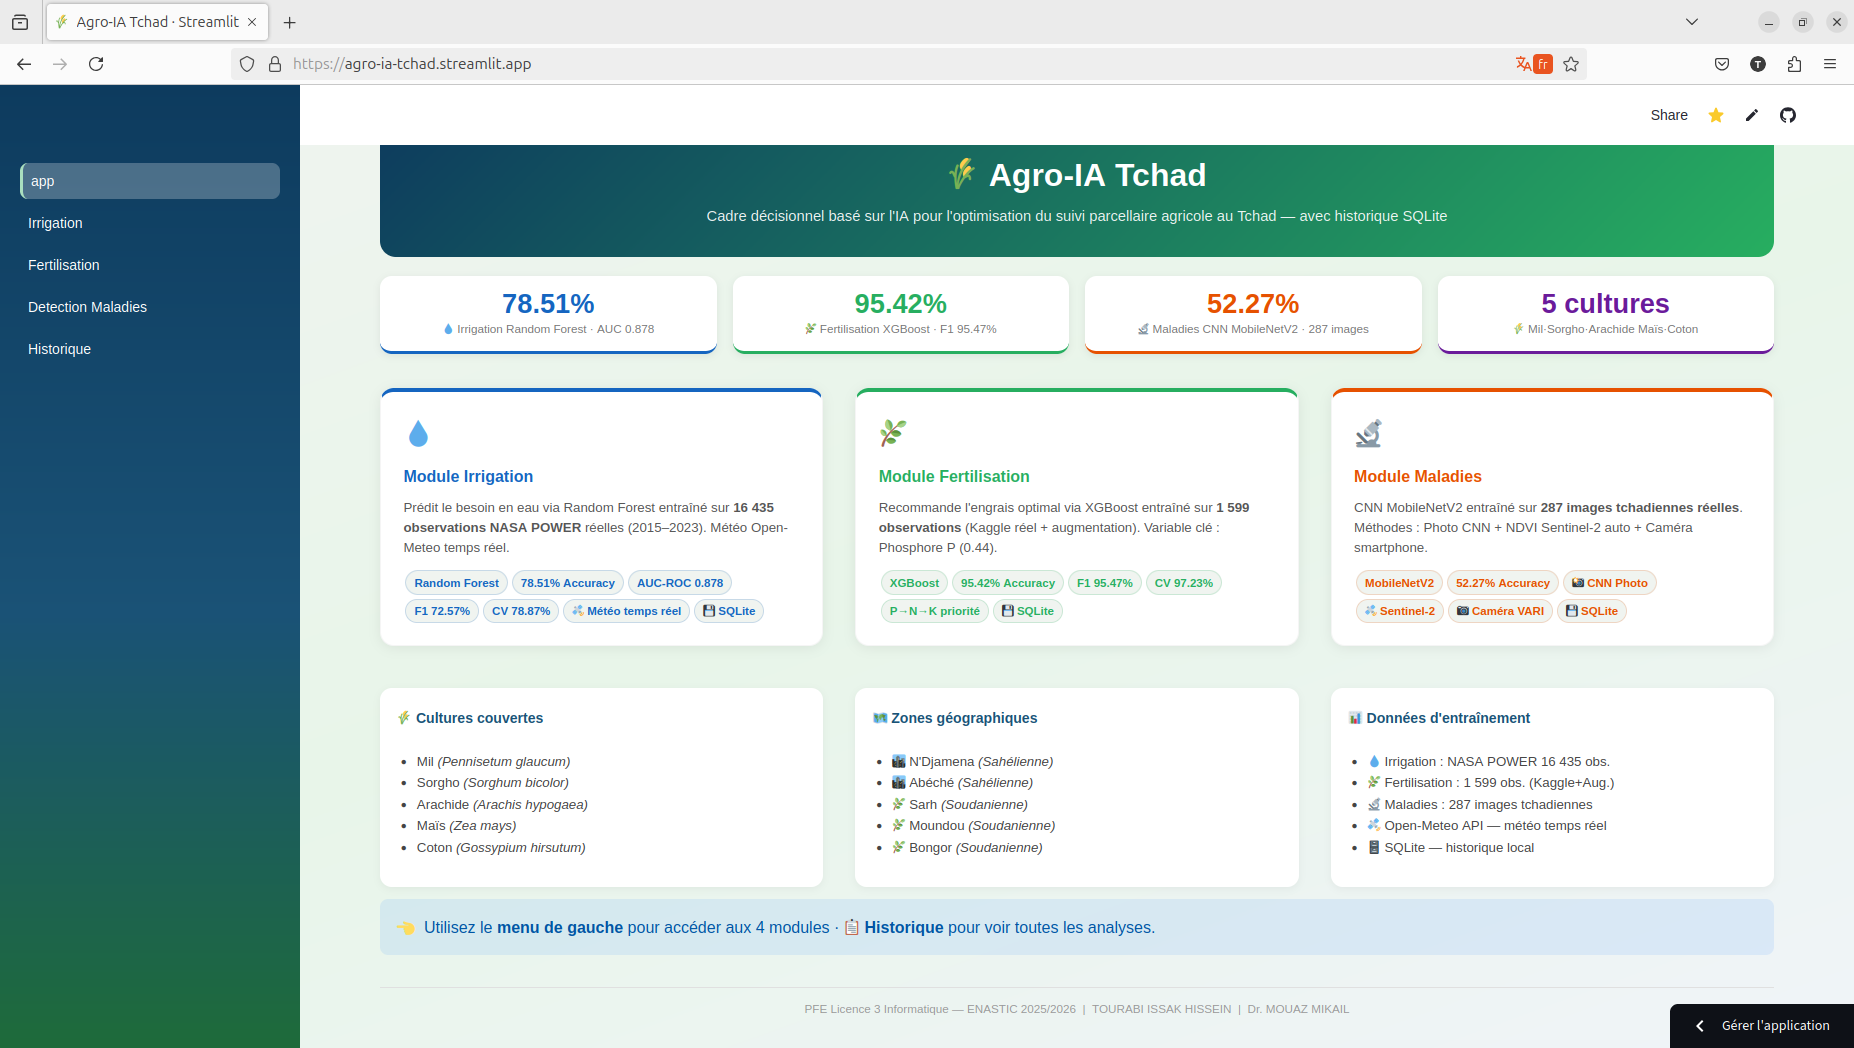
\includegraphics[width=0.9\textwidth]{images/capture_accueil.png}
	\fbox{\parbox{0.9\textwidth}{\centering\vspace{1.4cm}
			[Capture : page d'accueil --- métriques et statistiques]
			\vspace{1.4cm}}}
	\caption{Page d'accueil de l'application Agro-IA Tchad}
	\label{fig:cap_accueil}
\end{figure}

\begin{figure}[H]
	\centering
	% 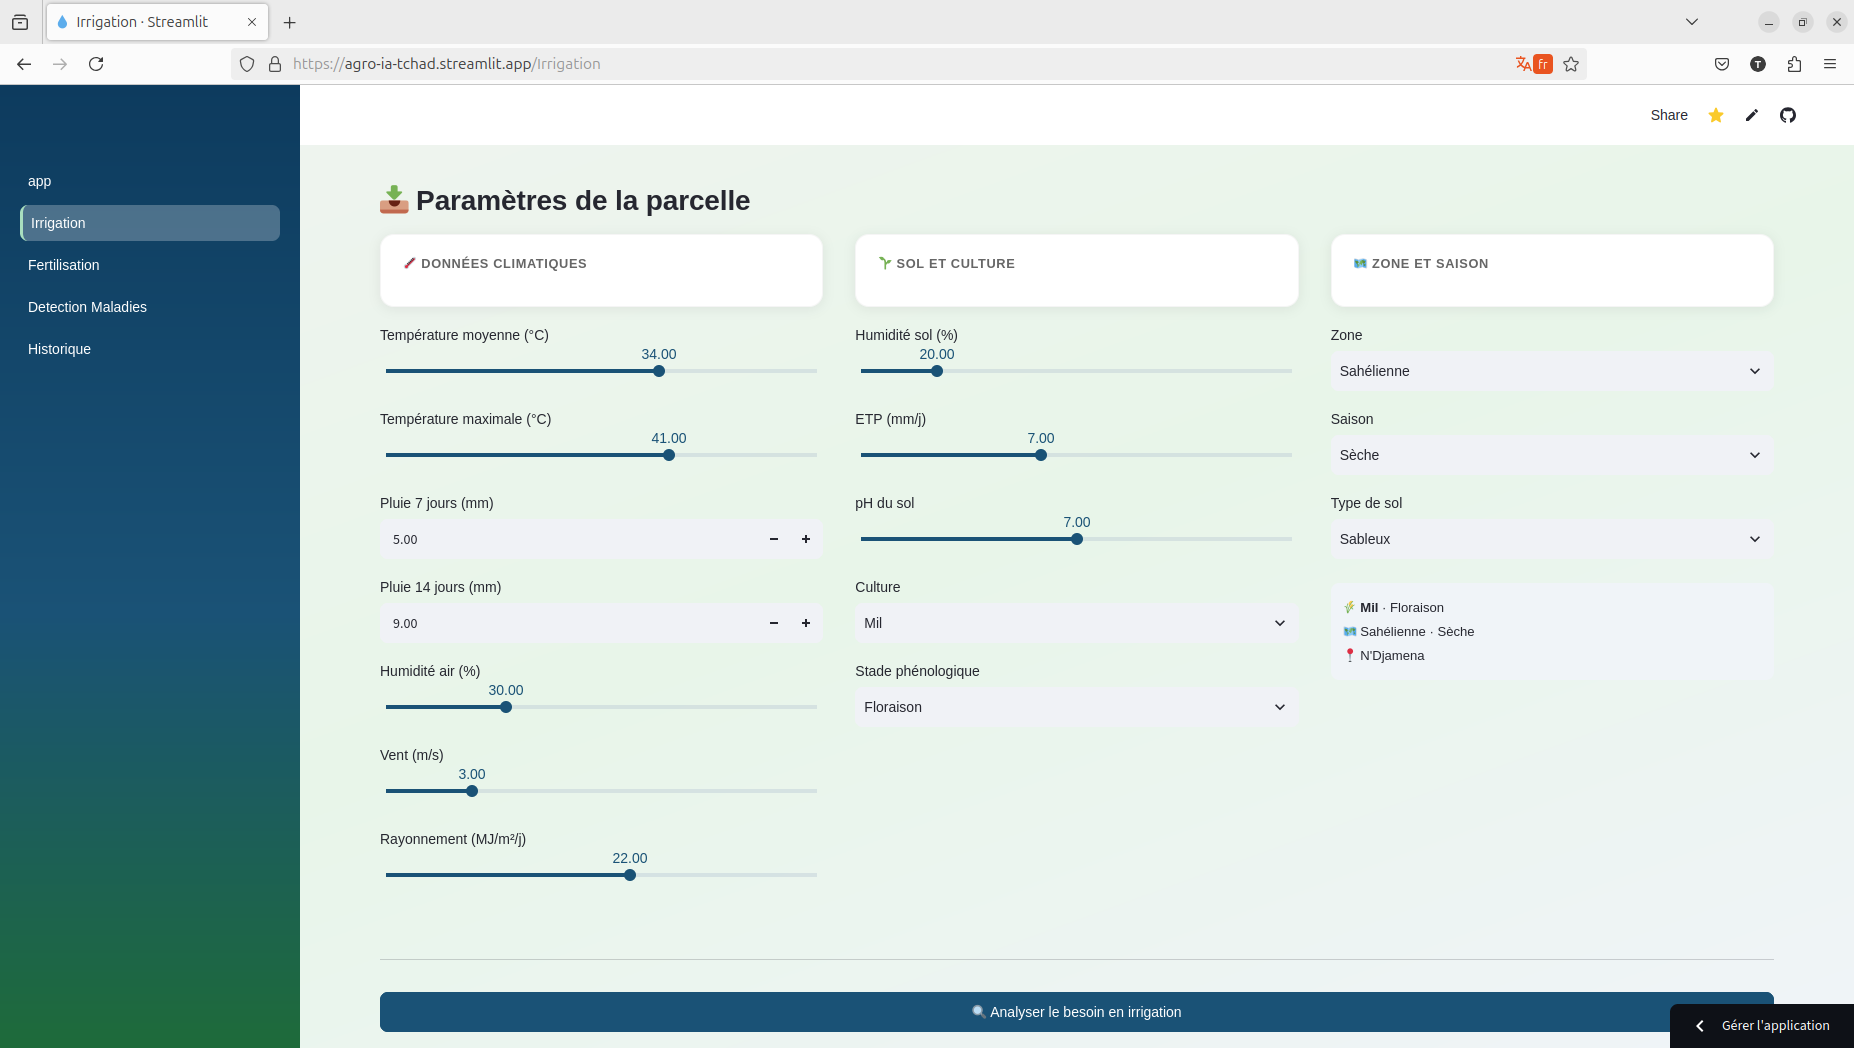
\includegraphics[width=0.9\textwidth]{images/capture_irrigation.png}
	\fbox{\parbox{0.9\textwidth}{\centering\vspace{1.4cm}
			[Capture : module Irrigation --- météo temps réel et résultat]
			\vspace{1.4cm}}}
	\caption{Module Irrigation --- analyse et recommandation}
	\label{fig:cap_irr}
\end{figure}

\begin{figure}[H]
	\centering
	% 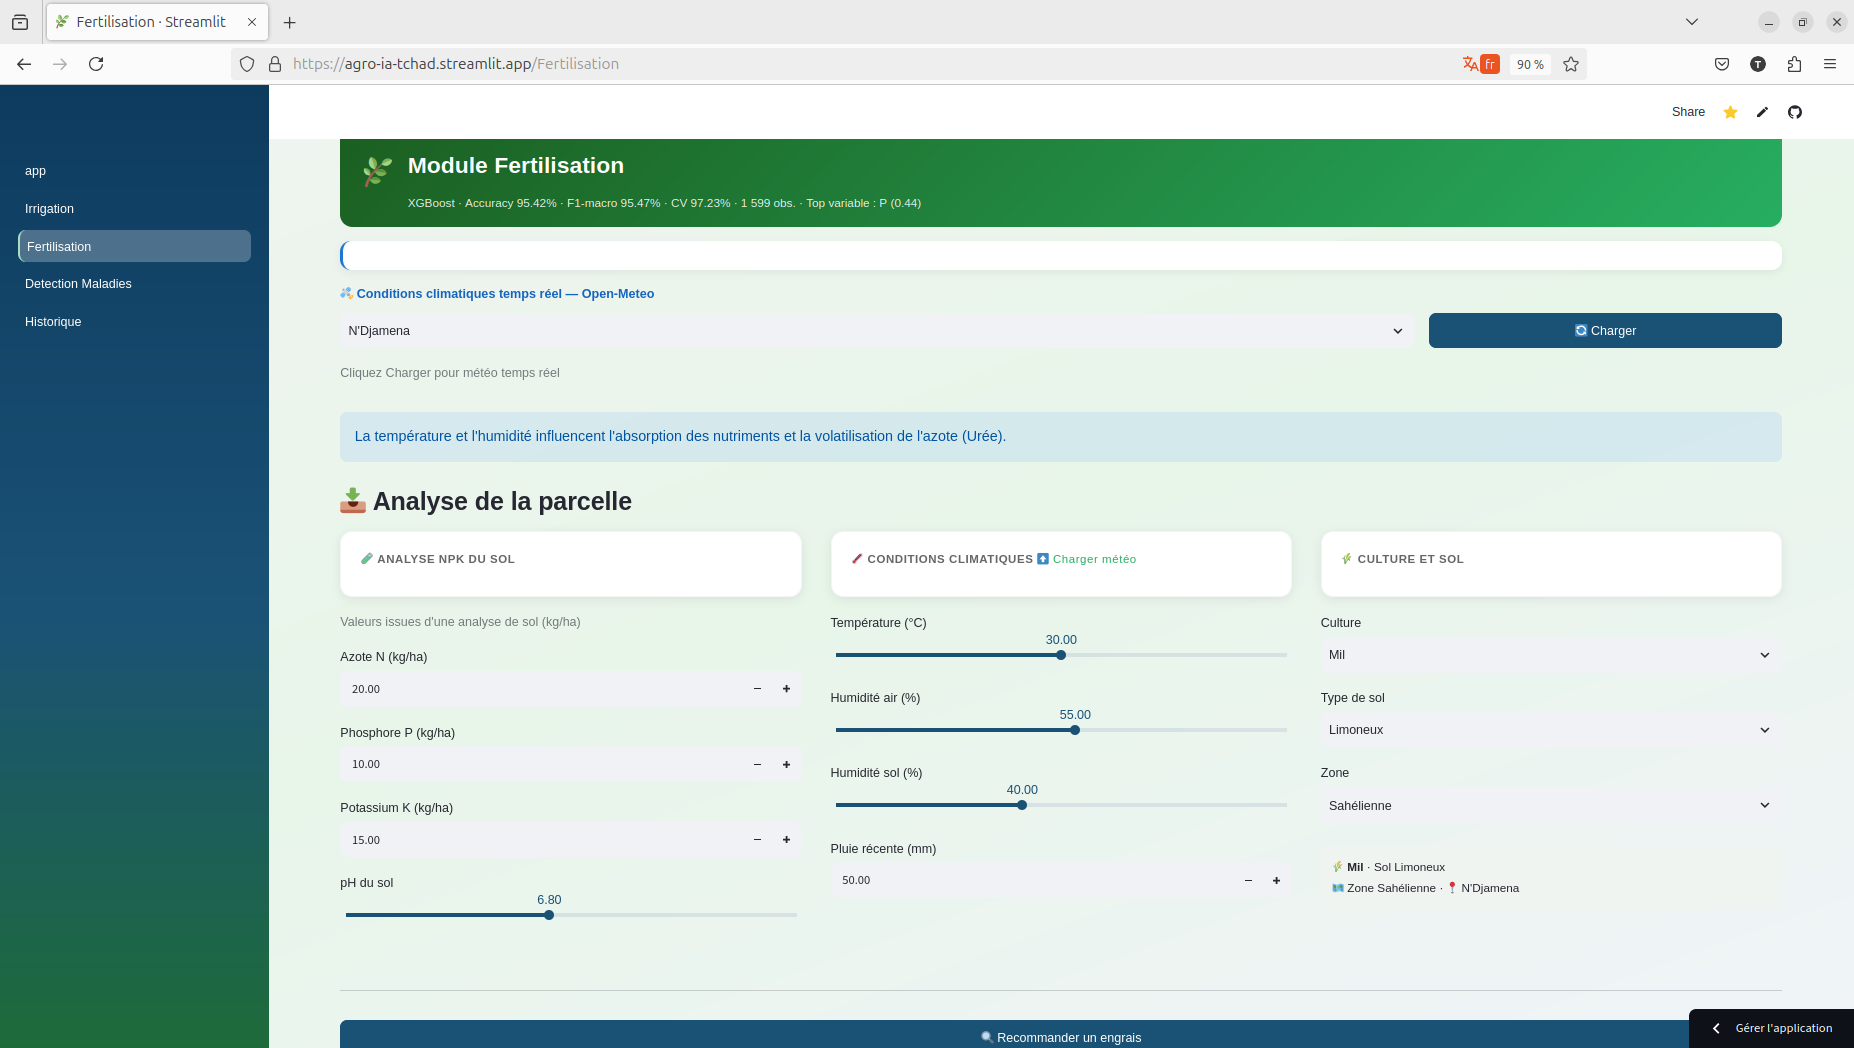
\includegraphics[width=0.9\textwidth]{images/capture_fertilisation.png}
	\fbox{\parbox{0.9\textwidth}{\centering\vspace{1.4cm}
			[Capture : module Fertilisation --- recommandation d'engrais]
			\vspace{1.4cm}}}
	\caption{Module Fertilisation --- recommandation d'engrais}
	\label{fig:cap_fert}
\end{figure}

\begin{figure}[H]
	\centering
	% 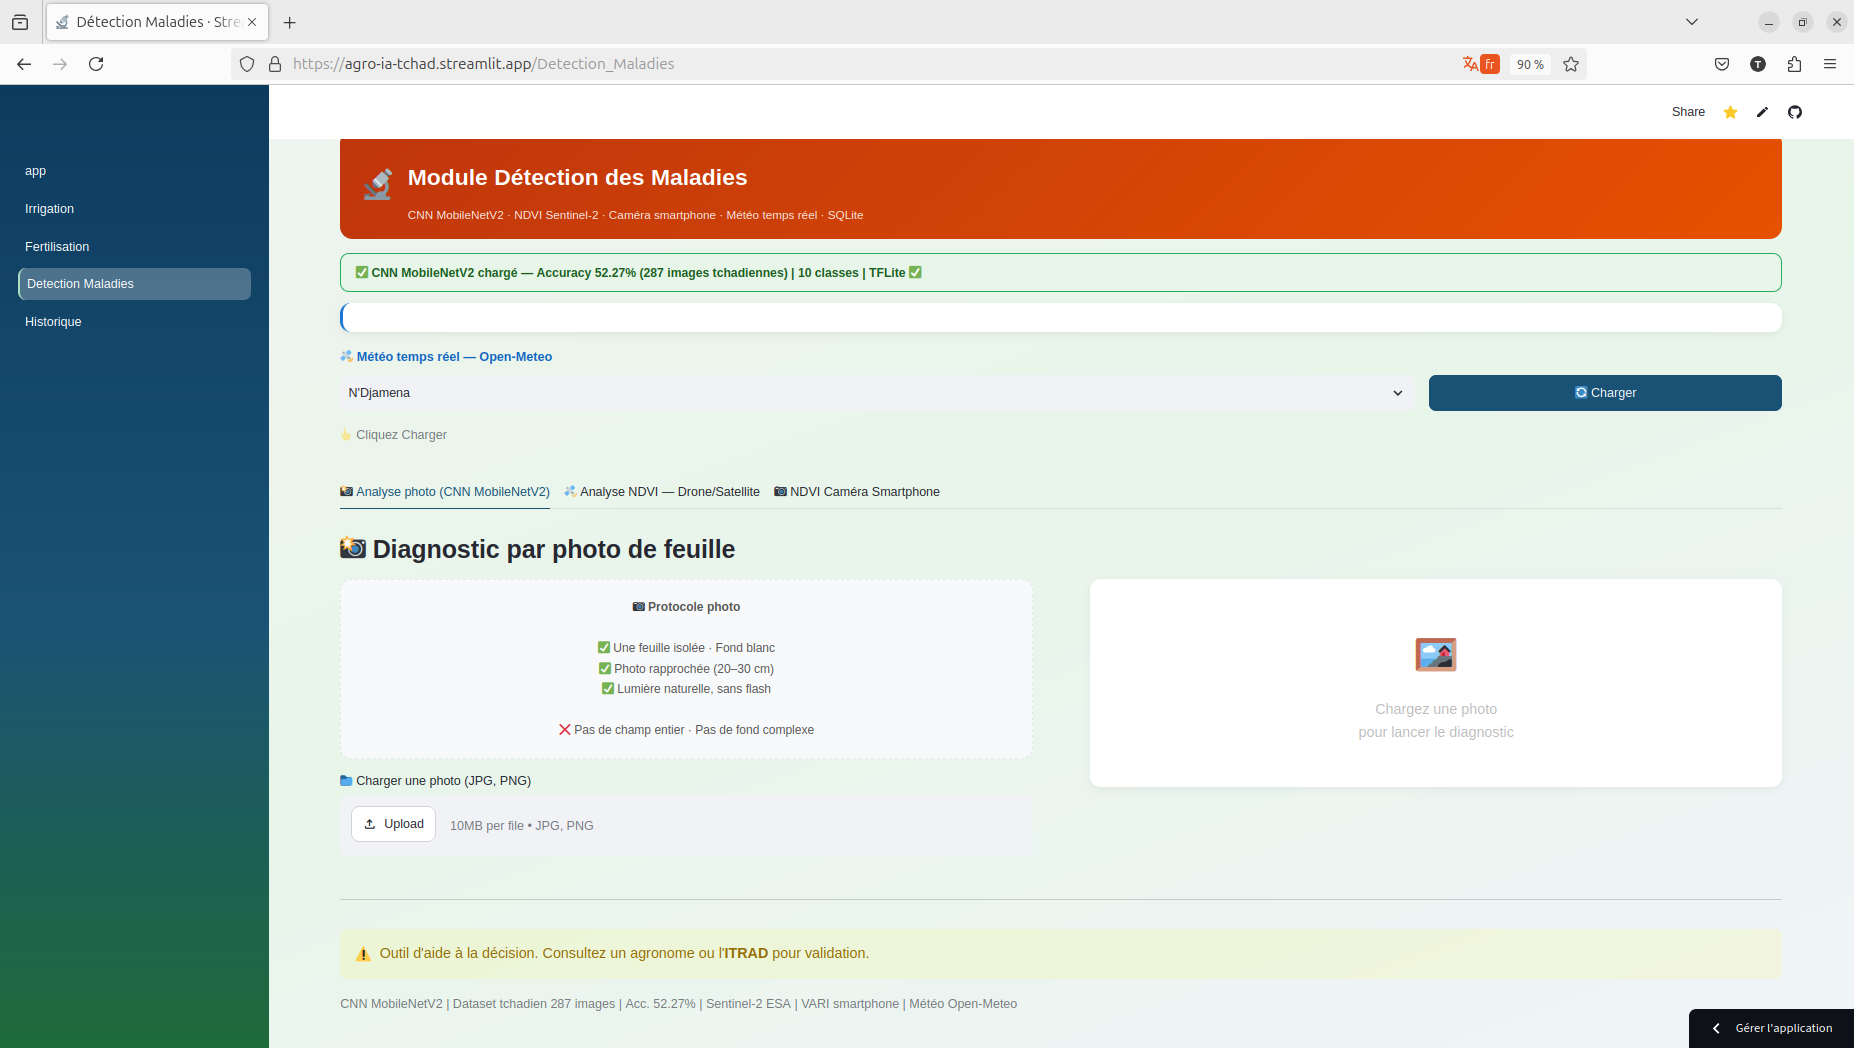
\includegraphics[width=0.9\textwidth]{images/capture_maladies.png}
	\fbox{\parbox{0.9\textwidth}{\centering\vspace{1.4cm}
			[Capture : module Maladies --- diagnostic CNN et NDVI]
			\vspace{1.4cm}}}
	\caption{Module Détection des maladies --- diagnostic par photo}
	\label{fig:cap_mal}
\end{figure}

\begin{figure}[H]
	\centering
	% 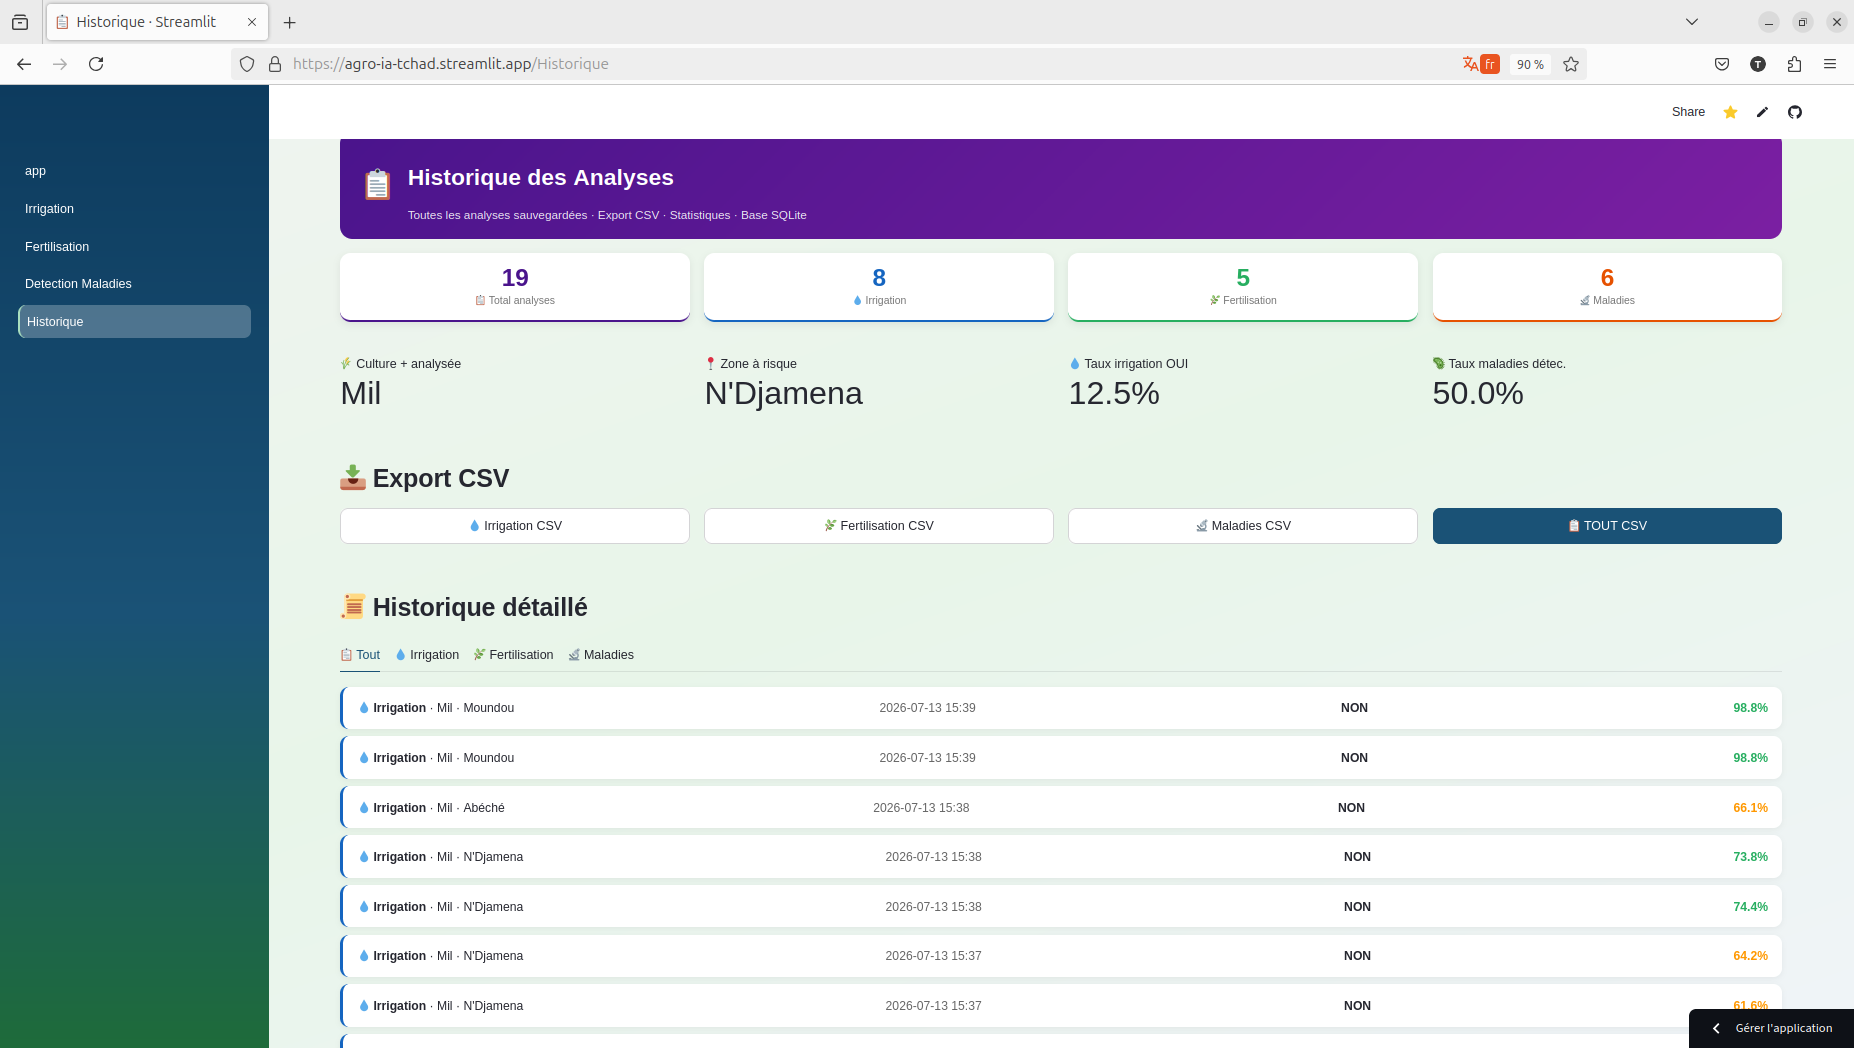
\includegraphics[width=0.9\textwidth]{images/capture_historique.png}
	\fbox{\parbox{0.9\textwidth}{\centering\vspace{1.4cm}
			[Capture : module Historique --- statistiques et export CSV]
			\vspace{1.4cm}}}
	\caption{Module Historique --- consultation et export}
	\label{fig:cap_hist}
\end{figure}
	\newpage
	
	% Table des matières complète (en dernier) — \tableofcontents
	% crée lui-même son titre ; pas de \chapter* supplémentaire.
	\clearpage
	\setcounter{tocdepth}{3}
	\phantomsection
	\addcontentsline{toc}{chapter}{Table des matières}
	\markboth{Table des matières}{Table des matières}
	\tableofcontents
	
\end{document}